\documentclass[11pt]{article}
\usepackage[margin=0.85in]{geometry}
\usepackage{amsmath,amssymb,graphicx,booktabs,longtable,array,xcolor,hyperref,fancyhdr,microtype}
\definecolor{ink}{HTML}{164D70}
\hypersetup{colorlinks=true,linkcolor=ink,urlcolor=ink,citecolor=ink}
\setlength{\parindent}{0pt}\setlength{\parskip}{6pt}
\setlength{\headheight}{15pt}
\pagestyle{fancy}\fancyhf{}\fancyhead[L]{\small Computational neurophysiology: frozen suite}
\fancyhead[R]{\small 18 October 2026}\fancyfoot[C]{\thepage}
\setcounter{topnumber}{2}\setcounter{bottomnumber}{2}
\renewcommand{\floatpagefraction}{0.65}
\newcommand{\R}{\mathbb{R}}
\emergencystretch=1em
\begin{document}
\title{\color{ink}Rule-dependent orientation judgement across a retention interval}
\author{Visual Attention and Working Memory Project\\Computational experiment series: previous trained model}\date{18 October 2026}\maketitle
\begin{abstract}
We characterized orientation cued in a frozen recurrent visual observer using behavioral challenges, spatial-priority interventions, memory perturbations and population decoding. Across 4 native conditions and 512 fresh trials, equal-condition accuracy was 99.8\% (95\% interval [99.4\%, 100.0\%]). For the representative condition D24, the strongest final answer readout among the tested regions was cls, with held-out macro AUC 1.000. The largest observed impairment in that condition was target\_\allowbreak{}-8\_\allowbreak{}evidence, changing accuracy by -56.2 percentage points. The analyses relate task competence to information availability, spatial selection and state dependence, with paired interventions and independent probe trials.
\end{abstract}
\section{Introduction and scientific questions}
This task combines a location instruction with a requested rotation sign. A positive report requires that the target rotate in the instructed direction. Target preservation, opposite rotation and distracting changes create competing sources of evidence, while blank intervals require the instruction and sample to persist.

We examine rotation magnitude, delay duration, cue-location decoding, remembered orientation and the final instructed response. The key mechanistic distinction is between preserving the visual sample and preserving the rule that determines how to interpret it. Time-generalization matrices ask whether readable information maintains a common population code across the delay.

The biological motivation is developed through \cite{spatial}, \cite{stokes}. The present experiments use the model as an accessible computational subject: its choices, internal population coordinates and interventions can be measured on exactly matched movies.

\subsection{Neuroscientific rationale}
Studies of dynamic prefrontal coding motivate tracking representations across the entire sequence rather than inspecting only a terminal state. The location and sign instruction can remain functionally available even while the pattern of recurrent activity changes. A decoder trained during one phase may therefore transfer well, poorly, or only after the relevant cue reappears. The time-generalization matrix tests this geometry explicitly. Resetting a state during the blank interval adds a causal test of maintenance: a subsequent performance loss identifies dependence on that state at a time when the task-relevant sample is absent.

% BEGIN BIOLOGICAL COMPARISON
\subsection{Biological experiments motivating this task}
\textbf{Experimental question.} How does a remembered orientation become a rule-dependent decision after a delay?

\paragraph{Harrison and Tong (2009)} Human fMRI patterns in V1-V4 identified the remembered grating orientation during a blank delay, including cases with little sustained average activation. Information in a population pattern could persist despite low mean activity. \cite{bio_harrison}

\paragraph{Griffin and Nobre (2003)} Cues presented before or after a visual array improved recognition of relevant locations. Behavioral and electrophysiological results linked orienting in perception and memory while revealing differences between precue and retrocue processing. \cite{bio_griffin}

\paragraph{Stokes and colleagues (2013)} Population analyses examined how prefrontal coding changed while establishing, maintaining and using task context. The study motivates measuring representational transformations through time rather than only mean persistent activation. \cite{bio_stokes}

These experiments motivate the behavioral, spatial-selection and population measurements reported below. The discussion returns to each study to compare its findings with the measured behavior and internal states of this observer.
% END BIOLOGICAL COMPARISON
\subsection{Task definition and prediction structure}
Did the target Gabor rotate in the direction requested by its location/sign glyph?

Response labels are 0: unchanged or opposite to cue sign; 1: rotation in cue sign. The native suite contains 4 conditions for this task. A complete condition table follows the main results. Detailed neural and intervention measurements use D24.

\subsection{Stimulus sequence and spatial layout}
For the representative native condition D24, the sequence has 28 frames, indexed from zero: frame 0: cue; frames 1--2: sample; frames 3--26: delay; frame 27: probe. The complete condition table specifies the other tested timing and difficulty settings.

The following values are observed in the 128 native trials of this representative condition. Continuous nuisance ranges summarize those draws.
\begin{center}\small\begin{tabular}{p{.56\textwidth}p{.34\textwidth}}\toprule Stimulus property & Observed values\\\midrule
Rotation magnitude (degrees) & 15, 30, 45\\
\bottomrule\end{tabular}\normalsize\end{center}
Stimulus centers in the 100 by 100 input are [[27.0, 27.0], [73.0, 27.0], [27.0, 73.0], [73.0, 73.0]]. Coordinate x increases rightward and y downward.

Attention manipulations are separated by encoding, delay and evidence epochs. Encoding interventions can alter what enters memory; delay interventions can change ongoing selection and memory writes; probe interventions can alter which comparison influences the decision. A reciprocal target cost and distractor benefit would support competitive spatial selection.


\section{Methods}
\subsection{Computational subject and experimental units}
The experimental subject is the previously trained 19-task model, with the main analysis fixed at update 204,289. This checkpoint was selected by the existing equal-task monitoring criterion before the present analysis. Its SHA-256 identifier is recorded in the reproducibility table. The final saved checkpoint at update 220,637 provides a matched robustness comparison. Model parameters are frozen throughout these experiments. A trial is a freshly generated native movie, its prescribed response, and the model's output. Independent procedural draws provide the sampling unit; resampling intervals quantify uncertainty for this trained subject under the specified stimulus distribution.

The 19-task training stage inherited the 16-task backbone and output heads, added three search-task heads, and continued optimization with Adam at learning rate $3\times10^{-4}$, moment coefficients $(0.9,0.999)$, numerical epsilon $10^{-8}$ and no weight decay. Effective batches contained 32 trials, accumulated in microbatches of four. The objective combined terminal cross-entropy with a 0.05-weighted pixel-prediction loss; VDA terminal cross-entropy additionally used the native reward value divided by three. Active-parameter gradient norm was clipped at 100. The selected checkpoint was saved during two-times static-memory-search sampling; the final checkpoint includes later four-times sampling. Checkpoint indices refer to this continuation stage, which itself inherited earlier learning.

Each native condition receives 128 new test trials. The final-checkpoint comparison replays the first 32 of those movies under the same generator namespace. Probe fitting uses 192 separate validation-split trials per selected condition and evaluation uses 128 test-split trials. Natural-image probe fitting and evaluation retain separate source-image splits. The native four-trial generator calls are preserved even when their tensors are combined into eight-trial GPU forwards. Inference uses float32; dense appearance, fusion and spatial recordings are stored in float16, while global memory, comparison memory and probabilities retain float32. Stimulus metadata defines analyses and interventions; only native pixels and the requested task head enter the observer's ordinary forward computation.

\subsection{Architecture and recording sites}
At each model frame, a 100 by 100 RGB (red, green and blue) image is represented at 100 sites arranged on a 10 by 10 grid. Each site carries 32 learned appearance channels, local RGB and contrast statistics, and temporal correspondence-derived features. A learned linear fusion maps these to 64 channels. The spatial recurrent state has 64 channels at each grid site; the global recurrent state, denoted $c_t$ and called CLS memory in the code, has 64 channels. CLS denotes the global classification-token pathway. A separate 735-dimensional comparison-memory vector accumulates selected local temporal-comparison evidence. The task head reads a learned 64-dimensional transformation of the concatenated global and comparison memories.

Let $v_{t,s}$ be the fused visual vector at site $s$, $h_{t-1,s}$ the preceding spatial memory, and $c_{t-1}$ the preceding global memory. The key and query are
\begin{align}
 k_{t,s}&=\operatorname{unit}\{W_k[\operatorname{LN}_v(v_{t,s})+\operatorname{LN}_h(h_{t-1,s})]\},\\
 q_t&=\operatorname{unit}\{W_q\operatorname{LN}_q(c_{t-1}+e_{\rm CLS})\},\\
 \ell_{t,s}&=\kappa\,k_{t,s}^{\mathsf T}q_t,\qquad
 \alpha_{t,s}=\frac{\exp\ell_{t,s}}{\sum_{u=1}^{100}\exp\ell_{t,u}}.
\end{align}
Here $W_k,W_q$ are learned matrices, $e_{\rm CLS}$ is a learned token vector, $\operatorname{LN}$ denotes layer normalization across channels, and $\operatorname{unit}$ divides a vector by its Euclidean norm with a numerical floor of $10^{-6}$. The expression $k^{\mathsf T}q$ is the key-query dot product. The scale is $\kappa=1+15\sigma(\rho)$, where $\rho$ is a learned scalar and $\sigma$ is the sigmoid function. Its value in the selected checkpoint is approximately 7.7525. The distribution $\alpha$ supplies the actual spatial-selection weights. There is one global query, so averaging the attention matrix over queries returns this same vector. The same spatial weights route learned visual values and temporal-comparison channels and influence spatial-memory writes.

Recordings are taken from appearance features, fused visual tokens, the spatial recurrent field, the global recurrent state, comparison memory and the attention distribution. We verify exact final-output and attention parity between the recording implementation and the authoritative model on all 19 tasks. Intermediate readouts are verified against forwards truncated at the corresponding frame. These controls establish that recording preserves the observer's original computation.

\subsection{Behavioral and signal-detection measures}
The model's response is the largest terminal class probability. Accuracy is the fraction of prescribed responses selected. Balanced accuracy averages recall across response classes. Macro AUC averages one-versus-rest receiver-operating-characteristic areas using continuous probabilities. Each native condition receives equal weight in the task summary. Wilson intervals accompany individual-condition accuracy; task intervals resample stimulus clusters within the fixed condition set. Matched procedural scenes remain together across timing conditions, and repeated photographs are grouped by image identity. A Wilson boundary interval is used when every observed response is correct or incorrect.

For binary judgements with both classes present, let $H$ and $F$ be hit and false-positive rates. With $h,f$ observed positive reports and $n_1,n_0$ opportunities, the finite-sample rates are $\widetilde H=(h+1/2)/(n_1+1)$ and $\widetilde F=(f+1/2)/(n_0+1)$. We report
\begin{equation}
 d'=\Phi^{-1}(\widetilde H)-\Phi^{-1}(\widetilde F),\qquad
 c=-\tfrac12[\Phi^{-1}(\widetilde H)+\Phi^{-1}(\widetilde F)].
\end{equation}
$\Phi^{-1}$ is the inverse standard-normal cumulative distribution. Sensitivity $d'$ measures separation under this signal-detection convention; criterion $c$ summarizes positive-response tendency. This scalar criterion is distinct from the time-indexed global-memory vector $c_t$. Labels and the meaning of a positive report are specified separately for each task. The Brier score in the condition tables is the trial-averaged sum $\sum_k[p(k)-\mathbf 1(y=k)]^2$, where $y$ is the prescribed class and $\mathbf 1(y=k)$ is one for that class and zero otherwise; smaller values indicate better probability predictions. Difficulty challenges use the existing audited renderers. Zero-strength observations retain their scheduled labels as an ambiguity control. The complete native factorial, empirical difficulty points and response probabilities are retained in machine-readable files.

\subsection{Threshold-defined chronometry}
The unchanged terminal readout is applied to each recorded prefix state. If $p_t(k)$ is its probability for class $k$, evidence becomes available at frame $t_0$, and $\theta$ is a fixed confidence threshold, then
\begin{equation}
 \tau_\theta=\min\{t-t_0+1:t\geq t_0,\ \max_k p_t(k)\geq\theta\}.
\end{equation}
The chosen class is the argmax at that first crossing. We use thresholds 0.6, 0.7, 0.8 and 0.9, fixed before inspection of outcomes. Trials without a crossing are right-censored at movie end. We report the crossing fraction, median frames among crossings, accuracy of crossing decisions and the fraction already above threshold before task evidence. Time is measured in model frames; two-observation tasks have only one post-evidence frame. This defines a reproducible computational commitment time for the trained readout.

\subsection{Spatial priority and causal manipulations}
Attention mass in a region $S$ is $A_t(S)=\sum_{s\in S}\alpha_{t,s}$. Spatial concentration is summarized by effective patch count, $N_{\rm eff}=\exp[-\sum_s\alpha_s\log\alpha_s]$, which equals 100 for a uniform distribution and approaches one for selection of a single patch. Spatial masks use model-site centers at pixel coordinates $4.5+10j$, where $j=0,\ldots,9$ on either axis. For point arrays, the designated mask surrounds the task-defined target center; the alternative is the next center in the renderer's location ordering, with wraparound. The radius is 16 pixels for search-array centers and 12 pixels for the other point arrays. Thus the alternative mask is a fixed geometric comparison location and need not coincide with the particular foil that changed. For VDA, masks contain the model-site centers mapped into each native cell by the exact nearest-neighbor resize; the alternative is the cell obtained by reversing the row-major cell index. Native VDA9 cues in this implementation occupy the two opposite corners, so these two masks are distinct. Full-field tasks use the top-left and bottom-right image quadrants as designated and alternative regions. Their designated sites are spatial test regions rather than inferred target objects. Off-site controls use a single site outside the two regional masks; the VDA control additionally minimizes Gabor occupancy.

Computational stimulation and inhibition add a signed dose $\delta$ to the priority logits at the selected sites and frames:
\begin{equation}
 \alpha^{(\delta)}_{t,s}=\operatorname{softmax}_s\{\ell_{t,s}+\delta\,\mathbf 1[s\in S]\mathbf 1[t\in E]\}.
\end{equation}
$E$ identifies encoding, delay or evidence frames. The indicator $\mathbf 1[\cdot]$ equals one when its condition holds and zero otherwise. Positive doses raise relative priority and negative doses lower it. The dose is measured in logit units. If a selected region has attention mass $A$ before adding a uniform regional dose, its immediate new mass is $A'=e^\delta A/(1-A+e^\delta A)$. Thus its odds against the remaining image are multiplied by $e^\delta$; a dose of four multiplies these odds by approximately 54.6. Later frames can additionally change through recurrent feedback. Evidence-epoch doses are $\pm2,\pm4,\pm8$ at designated and alternative sites; encoding and delay use $\pm4$. A missing epoch is explicitly recorded as zero active intervention trials. Off-site and global shifts provide controls. Every arm reuses identical input pixels. Adding the same constant to all logits must leave the softmax unchanged, and this invariance is checked during collection.

Memory manipulations replace one recurrent state by $g$ times that state after processing the middle delay frame, or after the frame immediately before evidence when no blank delay exists. The next frame is then processed from that modified state. Gains $g=0$ and $g=1.5$ respectively reset and amplify the global state, spatial state or comparison memory, one component at a time. The movie then continues normally. Paired accuracy differences compare each arm with the same-trial sham. Intervals use 3,000 paired resamples; zero-discordance outcomes use a conservative exact bound on the discordance probability, and all-gain/all-loss boundaries use Wilson intervals; exact discordant-pair binomial tests assess changes in correctness for independent procedural trials. For natural photographs, repeated probe or base-image identities remain grouped in bootstrap resamples, and 9,999 paired source-image sign flips test the accuracy contrast. The saved test-method field distinguishes those Monte Carlo cluster tests from the exact trial-level tests. Holm adjustment is applied within task, and the four designated $\pm4$ evidence comparisons also enter one family across tasks and selected conditions.

\subsection{Independent-trial decoding and population geometry}
Each region is transformed using probe-fitting trials only. Representations wider than 256 coordinates undergo a seeded, label-independent random projection to 256 dimensions. A fixed training-derived principal-component basis then retains at most 32 dimensions and is shared across time. Coordinates are standardized from the fitting data. This capacity-matched representation is used for external linear probes; the original agent remains frozen.

For a design matrix $X$, target matrix $Y$ and fixed ridge penalty $\lambda_{\rm ridge}=10$, the fitted mapping minimizes
\begin{equation}
 \|Y-XW-\mathbf 1 b^{\mathsf T}\|_F^2+\lambda_{\rm ridge}\|W\|_F^2.
\end{equation}
Each row of $X$ represents one trial and each column one retained activation coordinate. Each row of $Y$ contains that trial's desired decoding target. The matrix $W$ contains fitted weights and $b$ contains output intercepts; $\mathbf 1$ is a column of ones. The squared Frobenius norm $\|\cdot\|_F^2$ sums squared entries of a matrix. The first term therefore measures prediction error, while the second penalizes large fitted weights. Classification targets are one-hot answer labels, the model's eventual choice, and cue or target location where available. Continuous targets include an 8 by 8 RGB descriptor of the last sample/study image and circular orientation or motion variables when provided by the task. Continuous reconstruction is scored against a predictor using the fitting-set mean. The resulting $R^2$ can be negative when the fitted mapping predicts new trials worse than that baseline.

For the spatial and global recurrent states, a decoder fitted at each time is evaluated at every time on independent test trials. The vertical axis is training time and the horizontal axis is test time. Diagonal performance measures available information at the same phase; off-diagonal performance tests transfer of the fitted linear readout between phases. A final-time label-permutation test uses 199 fitting-label shuffles, with unchanged held-out labels. Population trajectories use the same training-derived axes, and their class means are computed from held-out trials. Participation ratio is $(\sum_j\lambda_j)^2/\sum_j\lambda_j^2$ for covariance eigenvalues $\lambda_j$ within the retained subspace. Frame-to-frame root-mean-square (RMS) displacement measures how rapidly the state evolves in those coordinates.
\subsection{Full-state controls and unit-level selectivity}
As a control for dimensionality reduction, external ridge classifiers are also fitted directly to every recorded coordinate at the final frame and at the memory-test frame (the middle blank-delay frame, or the frame immediately before evidence when no blank delay exists). The ridge penalty is selected from 0.001, 0.01, 0.1, 1 and 10 using a class-stratified 75/25 split inside the probe-fitting set. Standardization is fitted on the inner fitting subset during selection and on the full fitting set for the final held-out evaluation. Each standardized full-coordinate vector is additionally divided by the square root of its coordinate count; these penalty values refer to that normalized feature scale. The full-crop reconstruction and candidate-reconstruction regressions use the same scaling convention. These full-state probes supplement the fixed-capacity temporal analysis. Global-memory unit selectivity is assessed by response-class differences on held-out trials, with Holm correction across the 64 units. Cross-validated class-centroid distances multiply independently estimated fitting and test centroid differences, standardized by fitting-set channel dispersion; negative estimates are retained.

For native factorial summaries, bootstrap clusters retain the same procedural scene across matched timing conditions. Photo repeats are grouped by probe or base image identity within condition. This preserves the dependence generated by reusing stimuli. The saved condition-level results allow every marginal to be reconstructed and interactions to be examined directly.
\section{Results}
\subsection{Native behavior, difficulty and checkpoint robustness}
Native equal-condition accuracy was 99.8\%, with macro AUC 1.000. The matched final checkpoint changed accuracy by +0.78 percentage points on average across conditions, using 32 same-movie comparisons per condition. The lowest native cell was D24 at 99.2\%; the highest was D0 at 100.0\%. These comparisons retain the native sampling design rather than selecting trials after observing success.

In the empirical difficulty challenge, the smallest positive tested strength (2) produced 50.0\% correct responses, compared with 100.0\% at the largest strength (45). Each point uses 128 trials. The full curve, including intermediate levels and event-specific responses, is shown in Figure~\ref{fig:behavior}.

\begin{figure}[htbp]
\centering
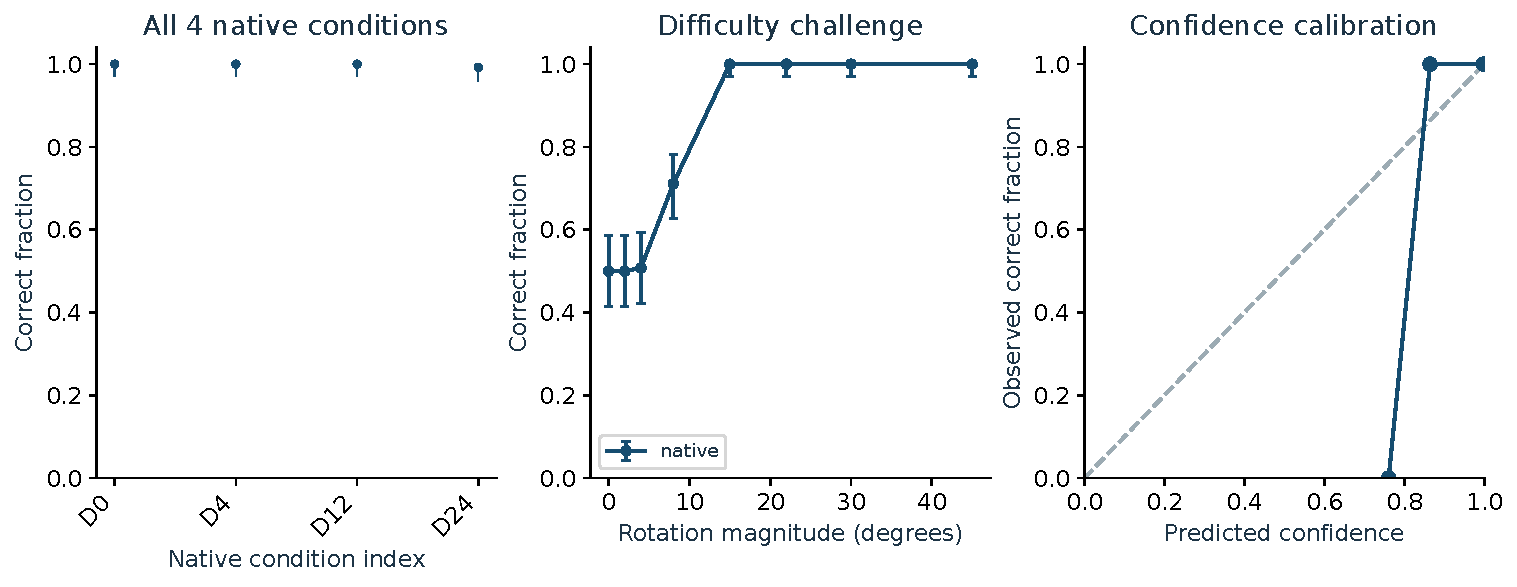
\includegraphics[width=.98\textwidth,height=.65\textheight,keepaspectratio]{../orientation_cued/figures/behavior.pdf}
\caption{\label{fig:behavior}Behavioral phenotype. Left: accuracy and Wilson intervals for every native condition. Middle: empirical signal-strength functions or native factorial margins. Right: observed accuracy within confidence bins, against the identity line. Zero-strength challenges assess responses to ambiguous physical evidence. Native cells contain 128 trials each.}
\end{figure}
\subsection{Exploratory psychometric threshold fit}
The native-label accuracy sweep is summarized by $P(x)=\gamma+(1-\gamma-\lambda)[1-\exp(-(x/a)^b)]$. Here $x$ is signal strength, $\gamma$ is reciprocal class count, $a>0$ sets scale, $b>0$ sets shape, and $\lambda\in[0,0.2]$ is the fitted lapse fraction. Binomial likelihood is minimized over the empirical levels. The midpoint threshold $x_{50}=a(\log 2)^{1/b}$ lies halfway between the guessing floor and fitted upper asymptote. This is an exploratory descriptive addition after observing the empirical curves. Three hundred bootstrap resamples retain the same nuisance-trial index across signal levels. Event-conditioned detection reports remain empirical. The approach follows the fitting and uncertainty principles discussed by Wichmann and Hill (2001; \url{https://pubmed.ncbi.nlm.nih.gov/11800458/}, \url{https://pubmed.ncbi.nlm.nih.gov/11800459/}).

The fitted midpoint was 8.373 task units (bootstrap interval [7.511, 8.841]), with slope 0.1067 probability per task unit and lapse 0.0\%. The largest absolute discrepancy from an observed point was 0.000. 

\begin{figure}[htbp]
\centering
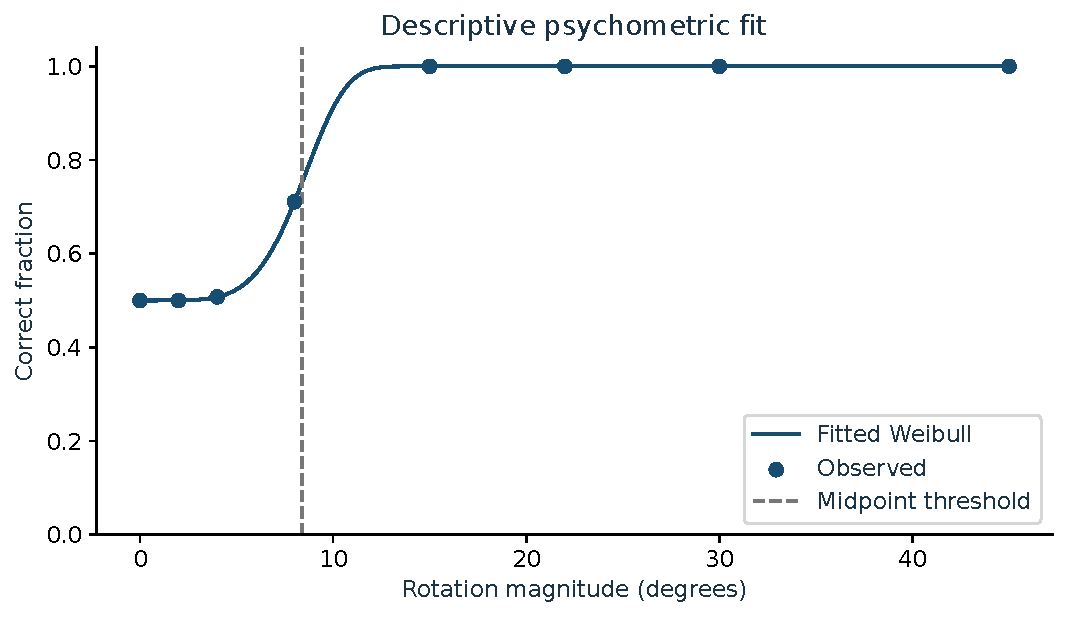
\includegraphics[width=.98\textwidth,height=.65\textheight,keepaspectratio]{../orientation_cued/figures/psychometric_fit.pdf}
\caption{Empirical points and descriptive Weibull function. The vertical line marks the midpoint between guessing and the fitted upper asymptote. Threshold units match the stimulus-strength axis.}
\end{figure}
\subsection{Time course and commitment thresholds}
\begin{center}\begin{tabular}{rrrrr}\toprule Threshold & Crossed & Median frames & Crossing accuracy & Premature\\\midrule
0.6 & 100.0\% & 1.0 & 99.2\% & 100.0\% \\
0.7 & 100.0\% & 1.0 & 99.2\% & 100.0\% \\
0.8 & 99.2\% & 1.0 & 100.0\% & 100.0\% \\
0.9 & 99.2\% & 1.0 & 100.0\% & 100.0\% \\
\bottomrule\end{tabular}\end{center}
The representative condition D24 provides 1 post-evidence frames. Median latency is conditional on crossing; the uncommitted-fraction plot retains all trials. The threshold sweep makes the speed--coverage tradeoff explicit. A rise in correct-answer probability over time can be compared with the development of location and answer decodability.

\begin{figure}[htbp]
\centering
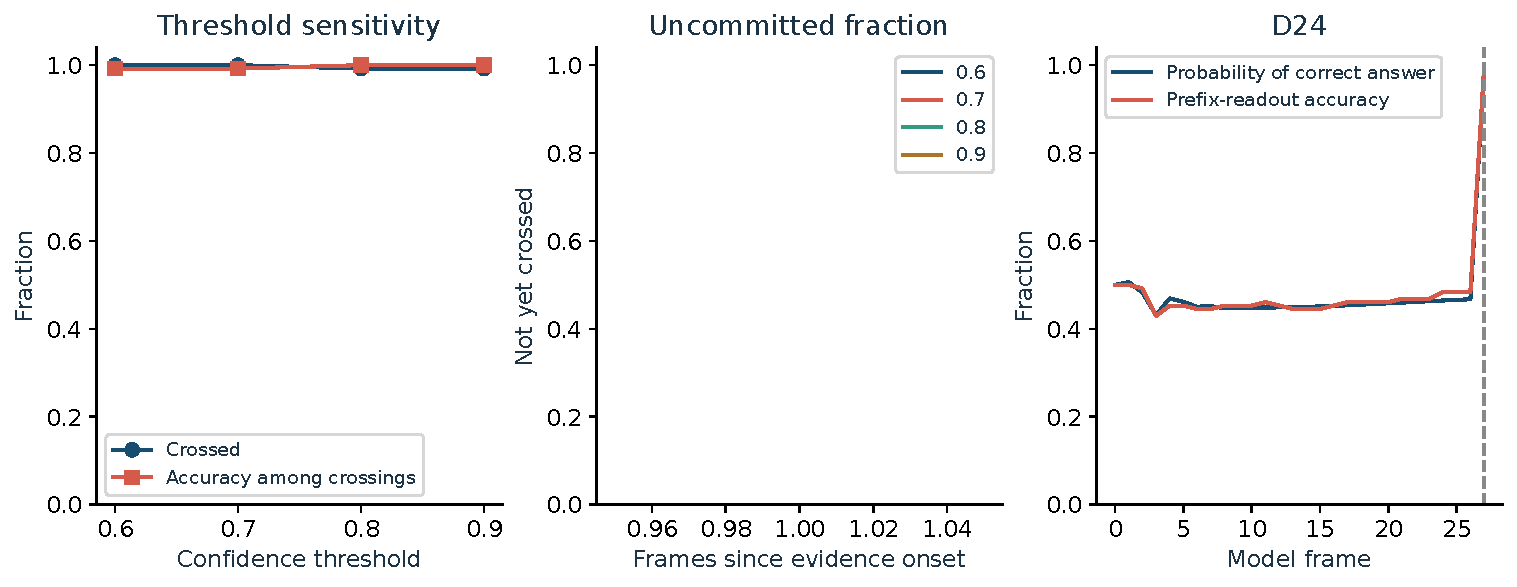
\includegraphics[width=.98\textwidth,height=.65\textheight,keepaspectratio]{../orientation_cued/figures/chronometry.pdf}
\caption{Threshold-defined timing. Left: the fraction reaching each confidence threshold and accuracy among those crossings. Middle: the fraction still uncommitted after each available evidence frame. Right: probability assigned to the correct response and accuracy of the unchanged head applied to prefix states. The dashed vertical line marks evidence onset.}
\end{figure}
\subsection{Does an early confident answer persist?}
A confidence threshold defines a hypothetical commitment rule. We test that rule directly by comparing its first post-evidence choice with the unchanged terminal choice on the same movie. A rescued error is an incorrect early commitment followed by a correct final answer; a spoiled answer changes from correct to incorrect. For four-class tasks, a revision can also exchange one incorrect alternative for another. These measurements determine whether terminal accuracy transfers to early stopping.

At threshold 0.8 across all native presentations, 511 of 512 trials crossed. Of those, 0 changed their answer later, 0 corrected an early error, and 0 lost an initially correct answer. These pooled counts are descriptive; the representative condition is shown separately below.

\begin{figure}[htbp]
\centering
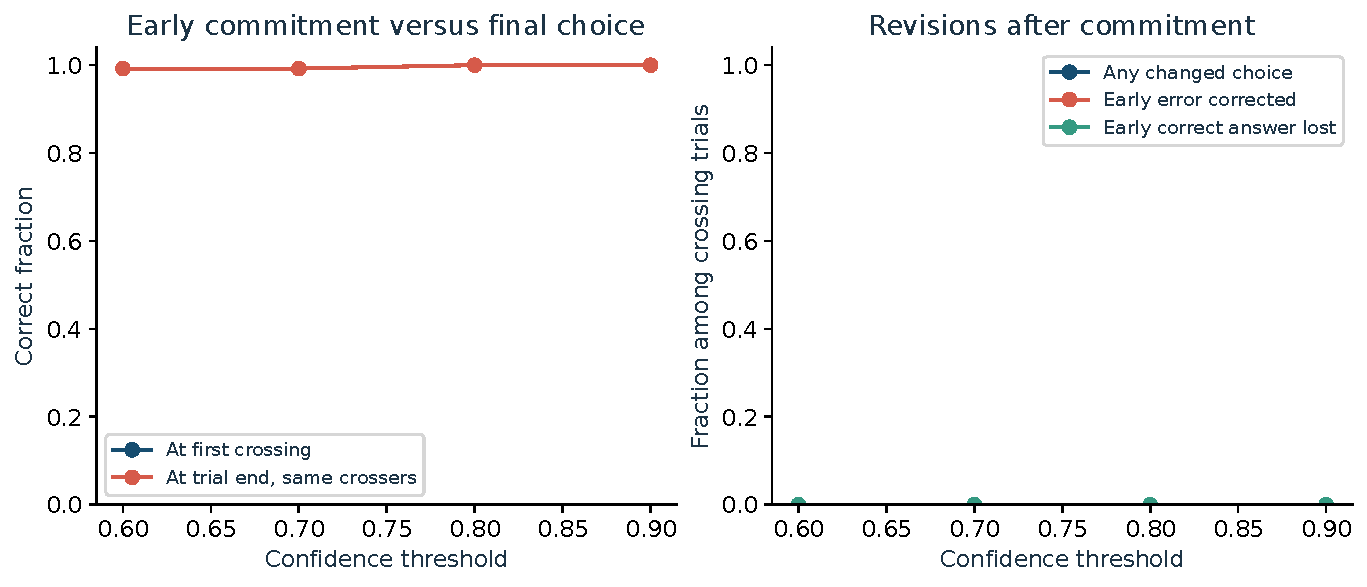
\includegraphics[width=.98\textwidth,height=.65\textheight,keepaspectratio]{../orientation_cued/figures/commitment.pdf}
\caption{Validity of first-threshold commitment in the representative native condition. Early and terminal accuracy are compared on exactly the same crossing trials at each threshold; the second panel separates kinds of later revision. Trials that never cross remain censored in the preceding analysis.}
\end{figure}
We additionally measure retrospective choice-settling latency: the first post-evidence frame from which the argmax remains equal to its terminal value for the rest of the movie. Frame counts start at one for the first available evidence frame. This measure uses future observations to locate the final revision. It describes the dynamics of the existing computation; it is distinct from the causal first-threshold stopping rule. Terminally correct and incorrect trajectories are kept separate.

\begin{figure}[htbp]
\centering
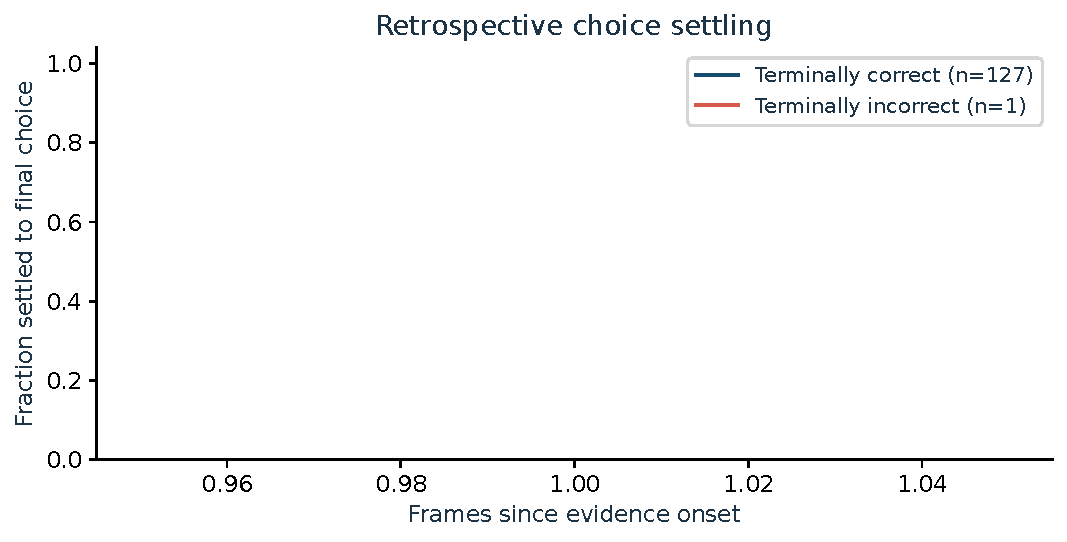
\includegraphics[width=.98\textwidth,height=.65\textheight,keepaspectratio]{../orientation_cued/figures/choice_settling.pdf}
\caption{Cumulative distribution of retrospective choice-settling times in the representative condition. A choice is settled once all subsequent prefix classifications agree with the terminal classification. Correct and incorrect terminal decisions can both settle, and are plotted separately.}
\end{figure}
% BEGIN CONDITION ATTENTION
\clearpage\subsection{Attention across conditions and time}
The analysis is organized around a direct visual question: where does the shared priority signal go as the trial unfolds, and how does that trajectory depend on the task condition? Rows retain fixed experimental conditions and physical locations. Columns follow time. The arrangement follows the heatmap-plus-time-course logic of Morgan, Albanna and Herman (2025), Figure 4 (\url{https://arxiv.org/html/2502.10955v1}).

The target is fixed at top left with a 24-frame delay. Rows separate target changes matching the instruction, unchanged targets, and target changes opposing the instruction. Clockwise and counterclockwise instructions are pooled.

\paragraph{What each plotted quantity means.}
For trial $i$, frame $t$ and image patch $p$, $\alpha_{itp}$ is the attention probability assigned to that patch; its sum over the 100 patches is one. For a condition containing $n$ trials, the map shows $\bar\alpha_{tp}=n^{-1}\sum_i\alpha_{itp}$. The 100 entries are placed back into their original 10-by-10 image grid without spatial rotation. A line for region $R$ shows the trial-average mass $M_R(t)=n^{-1}\sum_i\sum_{p\in R}\alpha_{itp}$. A line labeled ``other regions (mean) averages their separate masses rather than summing all alternatives. A dotted horizontal line marks the mass the same region would receive under uniform attention, its patch count divided by 100.

Target apertures use the same patch-center geometry throughout a task: circular masks with a 16-pixel radius for search arrays and a 12-pixel radius for the other localized tasks. VDA uses its native stimulus-cell boundaries mapped onto the 100-site grid. The central sample region is a 16-pixel-radius circle excluding candidate apertures. The source tables retain the exact region weights.

Every curve includes all selected trials, independently of whether the model answered correctly. Shaded bands are pointwise 95 percent intervals from 2,000 whole-trial bootstrap resamples. Repeated photograph identities are resampled together. These bands describe each condition separately. Phase-colored backgrounds mark encoding, retention and comparison; frame zero on the horizontal axis is the task-specific evidence onset, or the first motion transition in the duration task. Original frame numbers remain visible on the maps.

Map colors share one scale across every condition and time point within this task. A square-root color transform makes small weights visible; the colorbar retains probability units. The overview uses named temporal landmarks, with explicit original frame numbers when trial lengths differ. The appendix supplies every recorded frame, and the accompanying HTML viewer pairs an exact trial movie with its own attention overlay and the condition-average map.

\begin{center}\small\begin{tabular}{p{.68\textwidth}rr}\toprule Condition & Trials & Clusters\\\midrule
Matches instructed rotation & 16 & 16\\
Target unchanged & 11 & 11\\
Opposes instructed rotation & 5 & 5\\
\bottomrule\end{tabular}\normalsize\end{center}
\clearpage
\begin{figure}[htbp]
\centering
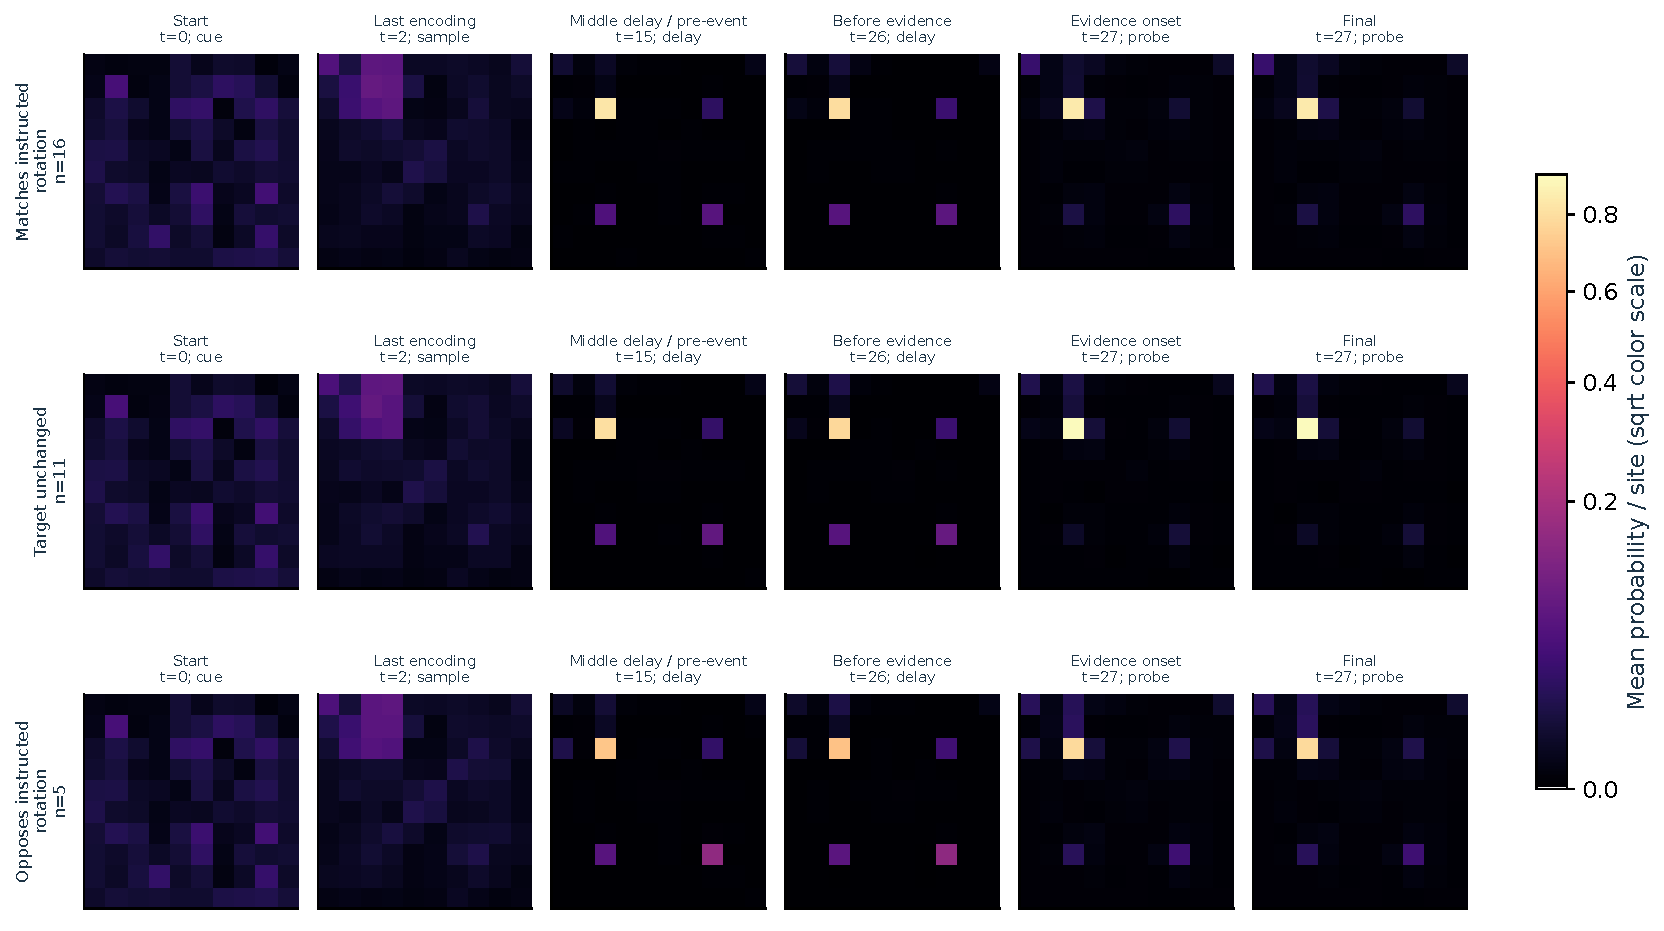
\includegraphics[width=.98\textwidth,height=.65\textheight,keepaspectratio]{../orientation_cued/figures/attention_conditions_landmarks_00.pdf}
\caption{Condition-by-time spatial allocation. Each row averages its stated trial group at a fixed physical location. The common square-root color scale is labeled in probability per patch. Original frame t and phase identify each observation; on full-series panels the signed number additionally gives time relative to evidence onset.}
\end{figure}
\clearpage
\begin{figure}[htbp]
\centering
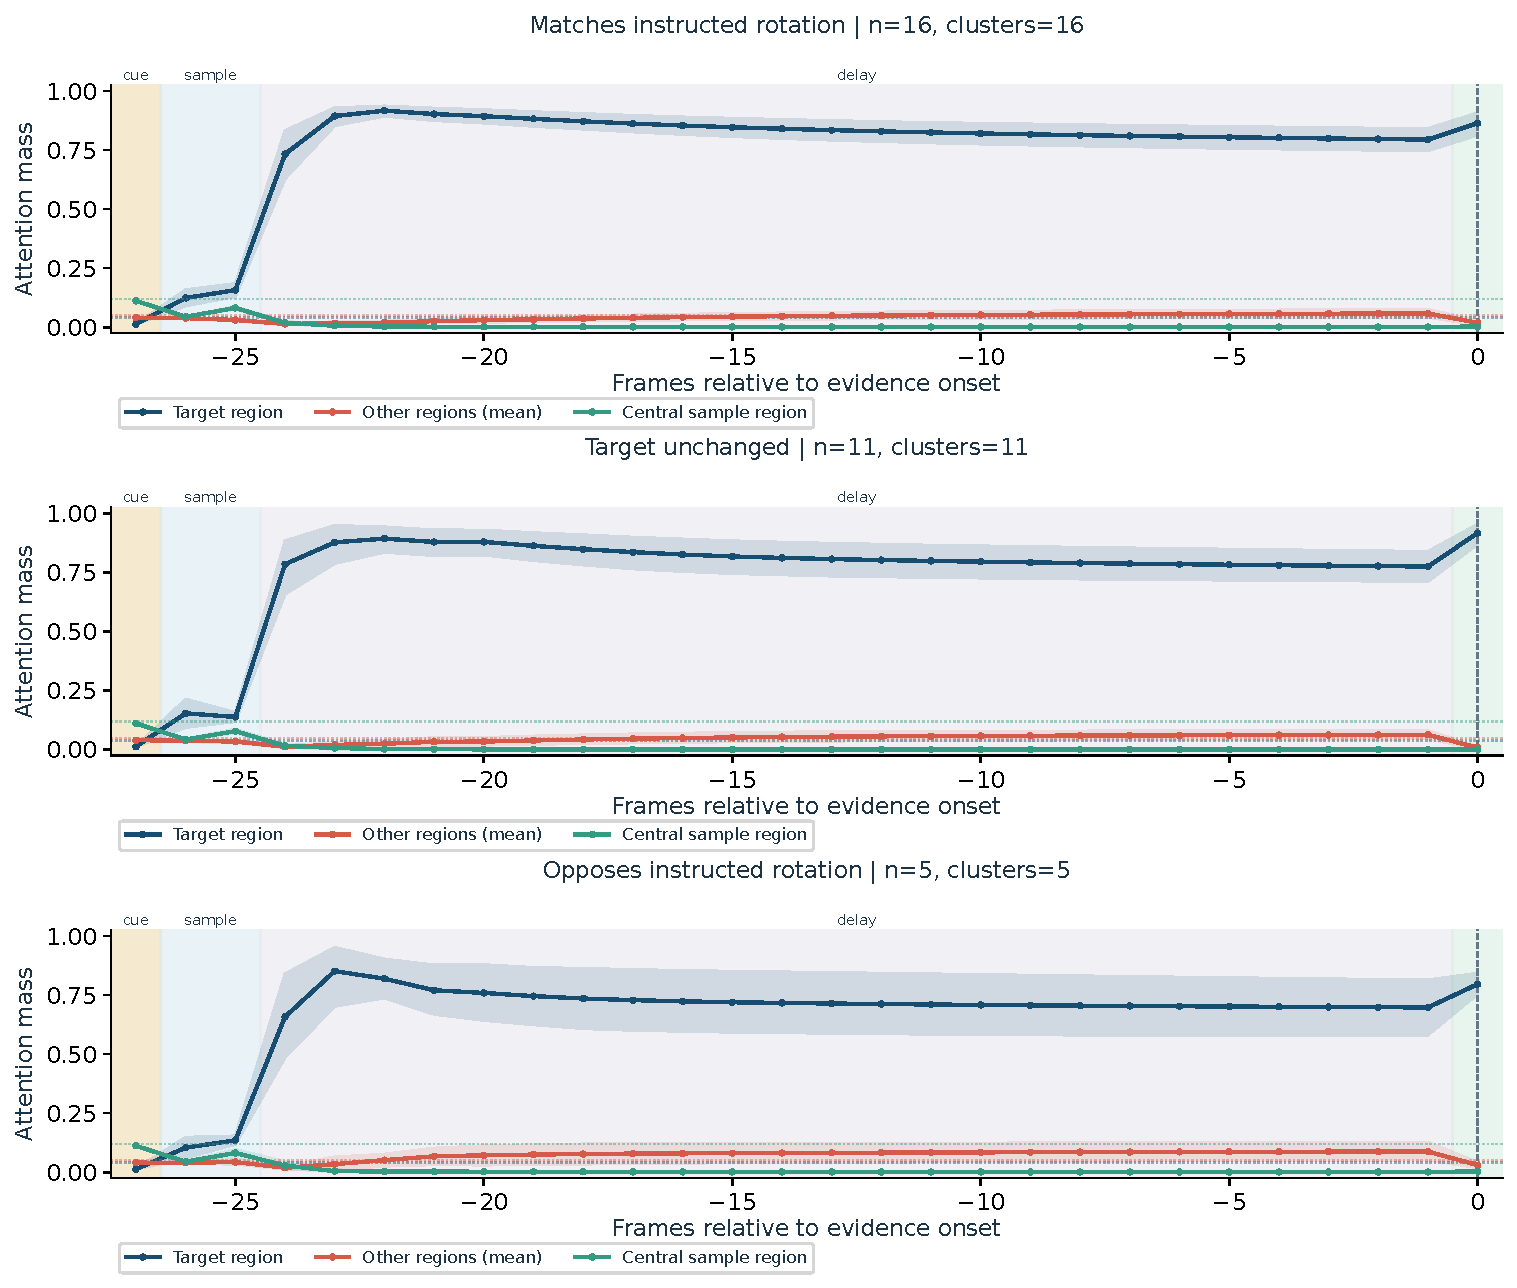
\includegraphics[width=.98\textwidth,height=.65\textheight,keepaspectratio]{../orientation_cued/figures/attention_conditions_curves_00.pdf}
\caption{Regional attention through the entire trial, separately for each condition. Solid traces are mean probability masses; shading gives pointwise 95 percent cluster-bootstrap intervals. Dotted lines show uniform allocation for each region. Background bands and labels identify trial phases. The vertical dashed line is the alignment event.}
\end{figure}
\clearpage
\begin{figure}[htbp]
\centering
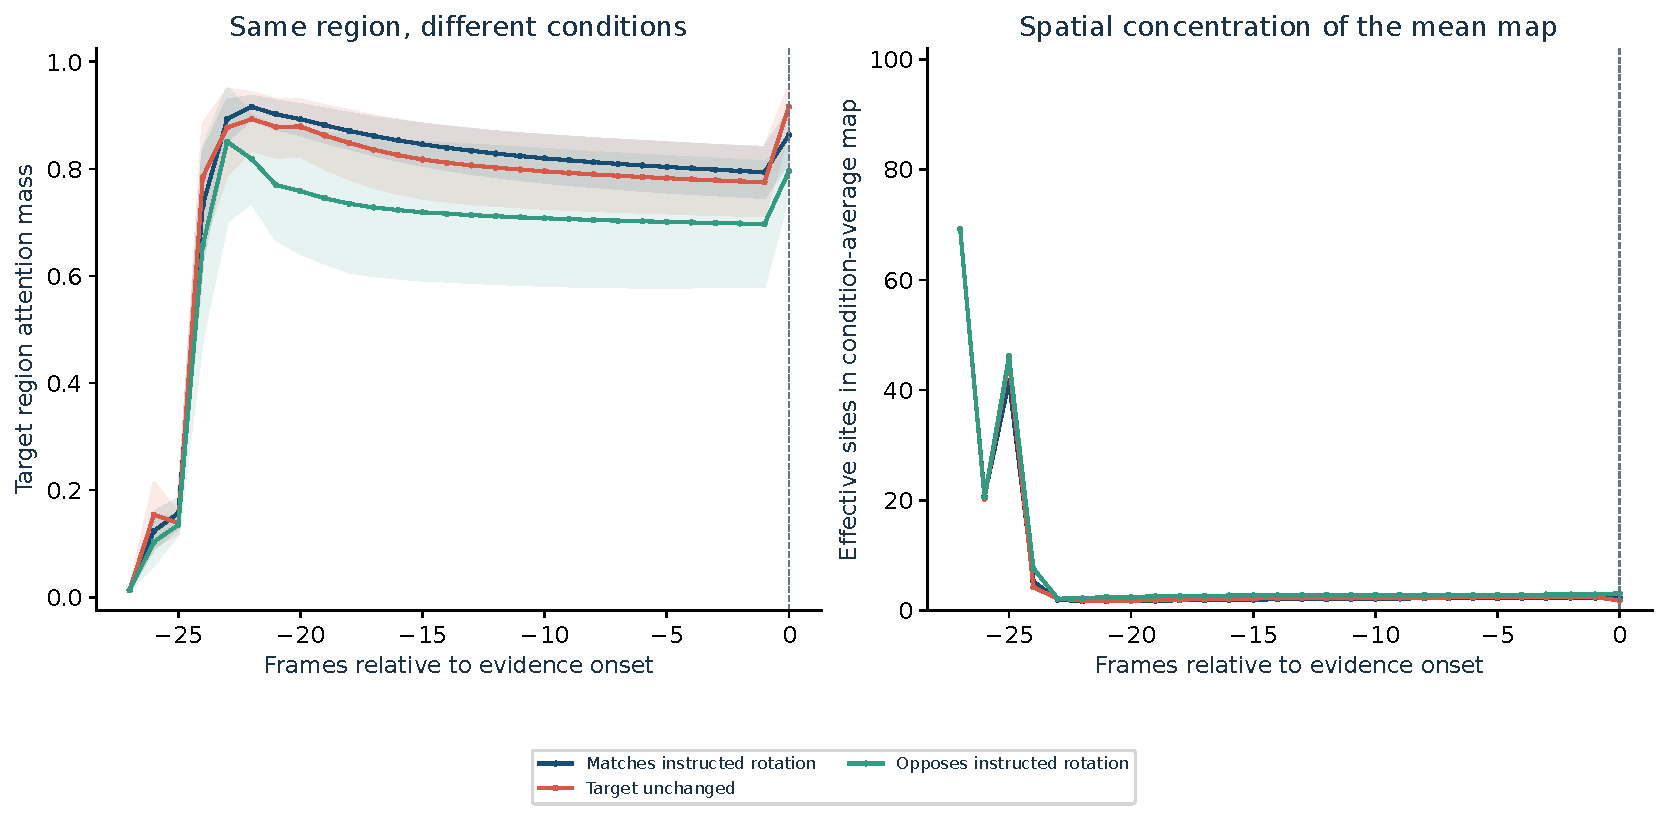
\includegraphics[width=.98\textwidth,height=.65\textheight,keepaspectratio]{../orientation_cued/figures/attention_conditions_compare.pdf}
\caption{Direct comparison of conditions on the same axes. Left: attention at the first named region, with pointwise uncertainty. Right: concentration of the condition-average map, measured as the exponential of its entropy. A value near 100 means a broad mean map; smaller values mean concentration on fewer sites. This summary is computed after averaging maps and is distinct from averaging each trial's concentration.}
\end{figure}
\paragraph{Reading the observed trajectories.}
Matches instructed rotation: target region mass peaks at 0.916 at original frame 5 (delay), and is 0.863 on the final frame. Target unchanged: target region mass peaks at 0.916 at original frame 27 (probe), and is 0.916 on the final frame. Opposes instructed rotation: target region mass peaks at 0.851 at original frame 4 (delay), and is 0.796 on the final frame. These summaries locate the observed allocation in time; the neighboring intervention experiments test its causal contribution to behavior.

% END CONDITION ATTENTION
\subsection{Causal sensitivity to spatial and mnemonic interventions}
For target\_\allowbreak{}-8\_\allowbreak{}evidence, paired accuracy changed by -56.2 percentage points (paired 95\% interval [-64.8\%, -47.7\%]; paired p=4.235e-22; within-task Holm p=1.313e-20). There were 0 corrected trials and 72 newly incorrect trials. For target\_\allowbreak{}-2\_\allowbreak{}evidence, paired accuracy changed by +0.0 percentage points (paired 95\% interval [-2.8\%, 2.8\%]; paired p=1; within-task Holm p=1). There were 0 corrected trials and 0 newly incorrect trials. These extrema describe the observed exploratory sweep. The four predesignated spatial comparisons at dose magnitude four are evaluated jointly across the full series in the integrated synthesis.

\begin{figure}[htbp]
\centering
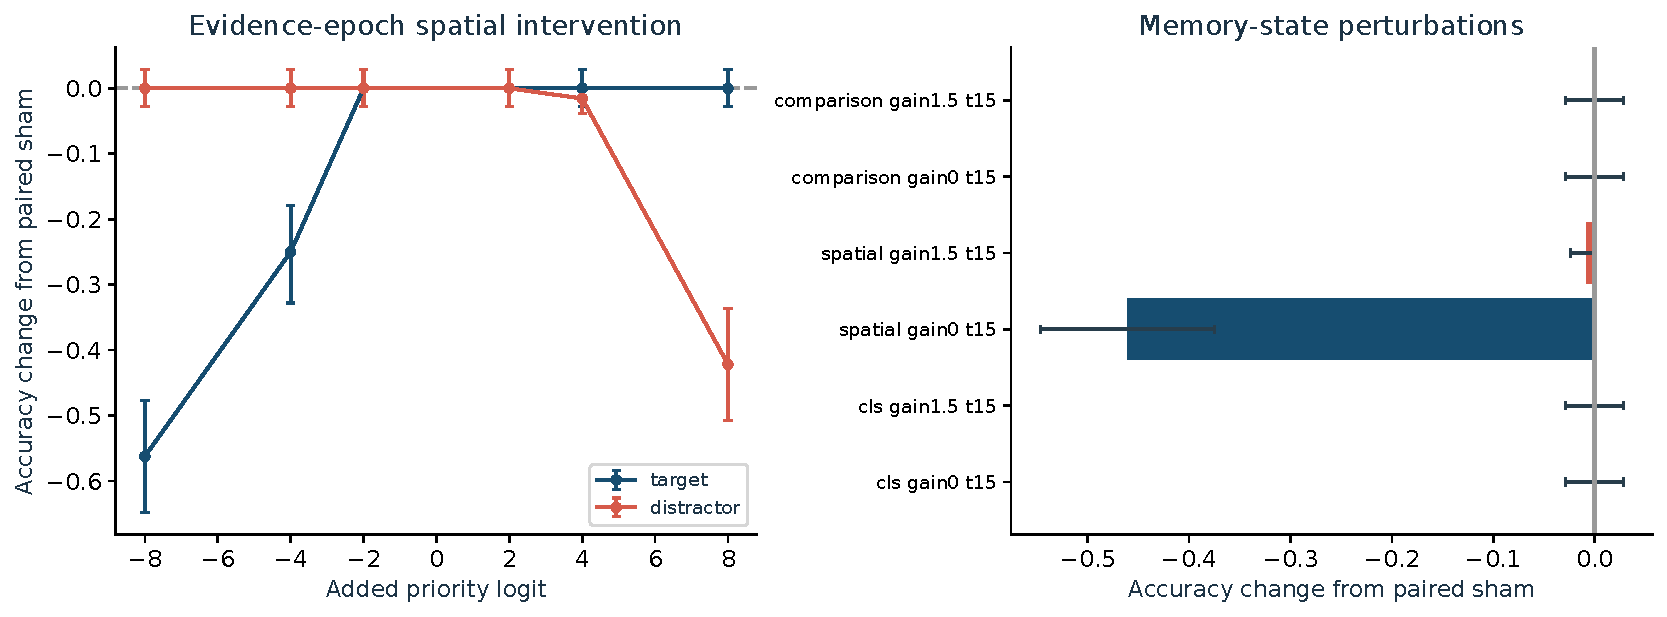
\includegraphics[width=.98\textwidth,height=.65\textheight,keepaspectratio]{../orientation_cued/figures/causal.pdf}
\caption{Matched causal effects in the representative condition. Left: changes from sham across signed spatial-priority doses during available evidence. Right: resetting or amplifying one memory component at the specified frame. Intervals resample matched trials, preserving sham--intervention pairing. Target and distractor labels denote the task geometry; full-field tasks use fixed quadrants.}
\end{figure}
\clearpage\subsection{Predesignated spatial comparisons across the full series}
The following dose-four evidence comparisons belong to one family of 108 tests across all nineteen tasks and selected conditions. The Holm-adjusted values therefore account for the complete primary spatial family. Positive changes indicate benefit and negative changes indicate impairment relative to the same-movie sham.

\small\begin{longtable}{p{.29\textwidth}p{.32\textwidth}rr}\toprule Condition & Intervention & Change (pp) & Global Holm p\\\midrule\endhead
D24 & target\_\allowbreak{}-4 & -25.0 & 4.051e-08\\
D24 & target\_\allowbreak{}+4 & +0.0 & 1\\
D24 & distractor\_\allowbreak{}-4 & +0.0 & 1\\
D24 & distractor\_\allowbreak{}+4 & -1.6 & 1\\
\bottomrule\end{longtable}\normalsize
\subsection{Readable information across representation levels}
\begin{center}\begin{tabular}{lrrr}\toprule Region & Final AUC & Balanced accuracy & Permutation p\\\midrule
appearance & 0.509 & 50.8\% & 0.525\\
fusion & 0.519 & 52.3\% & 0.350\\
spatial & 0.469 & 50.0\% & 0.555\\
cls & 1.000 & 100.0\% & 0.005\\
comparison & 0.455 & 46.1\% & 0.940\\
attention & 0.589 & 57.0\% & 0.020\\
\bottomrule\end{tabular}\end{center}
All table entries are evaluated on held-out trials. Final-time permutation p-values quantify how unusual the observed decoding is relative to shuffled fitting labels; the full regional panel is exploratory. The capacity-matched probes quantify readable information in the specified projected subspaces. Choice, location and continuous-feature targets are retained in the accompanying JSON results.

\begin{figure}[htbp]
\centering
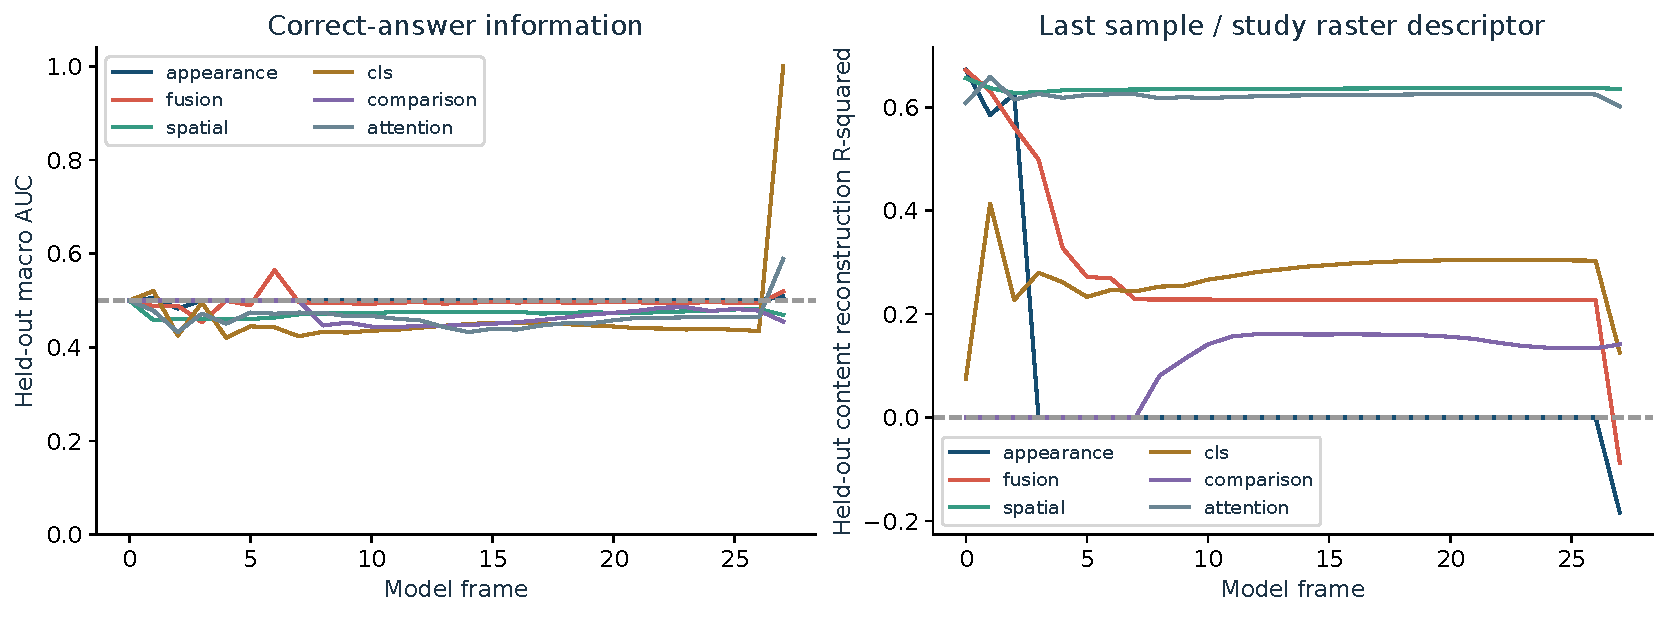
\includegraphics[width=.98\textwidth,height=.65\textheight,keepaspectratio]{../orientation_cued/figures/decoding.pdf}
\caption{Information across six recording sites. The answer-decoding curves report held-out macro AUC. Sample-content curves report reconstruction of a coarse last-sample or last-study image descriptor relative to a fitting-set-mean predictor. Each region uses an independently fitted training-only projection, shared across time; the agent itself is unchanged.}
\end{figure}
\subsection{Mnemonic population geometry and code stability}
In cls memory, the participation ratio ranged from 2.17 to 17.87 within the retained subspace. The final step displacement was 1.469 standardized RMS units. In spatial memory, the participation ratio ranged from 2.97 to 21.68 within the retained subspace. The final step displacement was 0.216 standardized RMS units. The time-generalization matrices distinguish a stable readout from information that is readable only by a phase-specific decoder. Broad off-diagonal AUC supports persistence of a common linear discriminant; a strong diagonal with weaker transfer supports changing code geometry. Trajectories use one set of axes fitted to independent fitting trials, so apparent movement is not caused by refitting the axes at each frame.

At memory-test frame 15, reconstruction of the sample orientation at the instructed location, represented by the cosine and sine of twice its angle had held-out R-squared 0.953 in CLS memory and 0.772 in spatial memory. This continuous target describes stimulus content, while the final-answer decoder tests the response required after the subsequent evidence.

At the same intervention boundary, resetting each component changed paired accuracy as follows: cls, +0.0 percentage points, spatial, -46.1 percentage points, comparison, +0.0 percentage points. Comparing these causal effects with the decoding curves distinguishes information that is recoverable from a state from information whose removal at that instant affects the subsequent choice.

\begin{figure}[htbp]
\centering
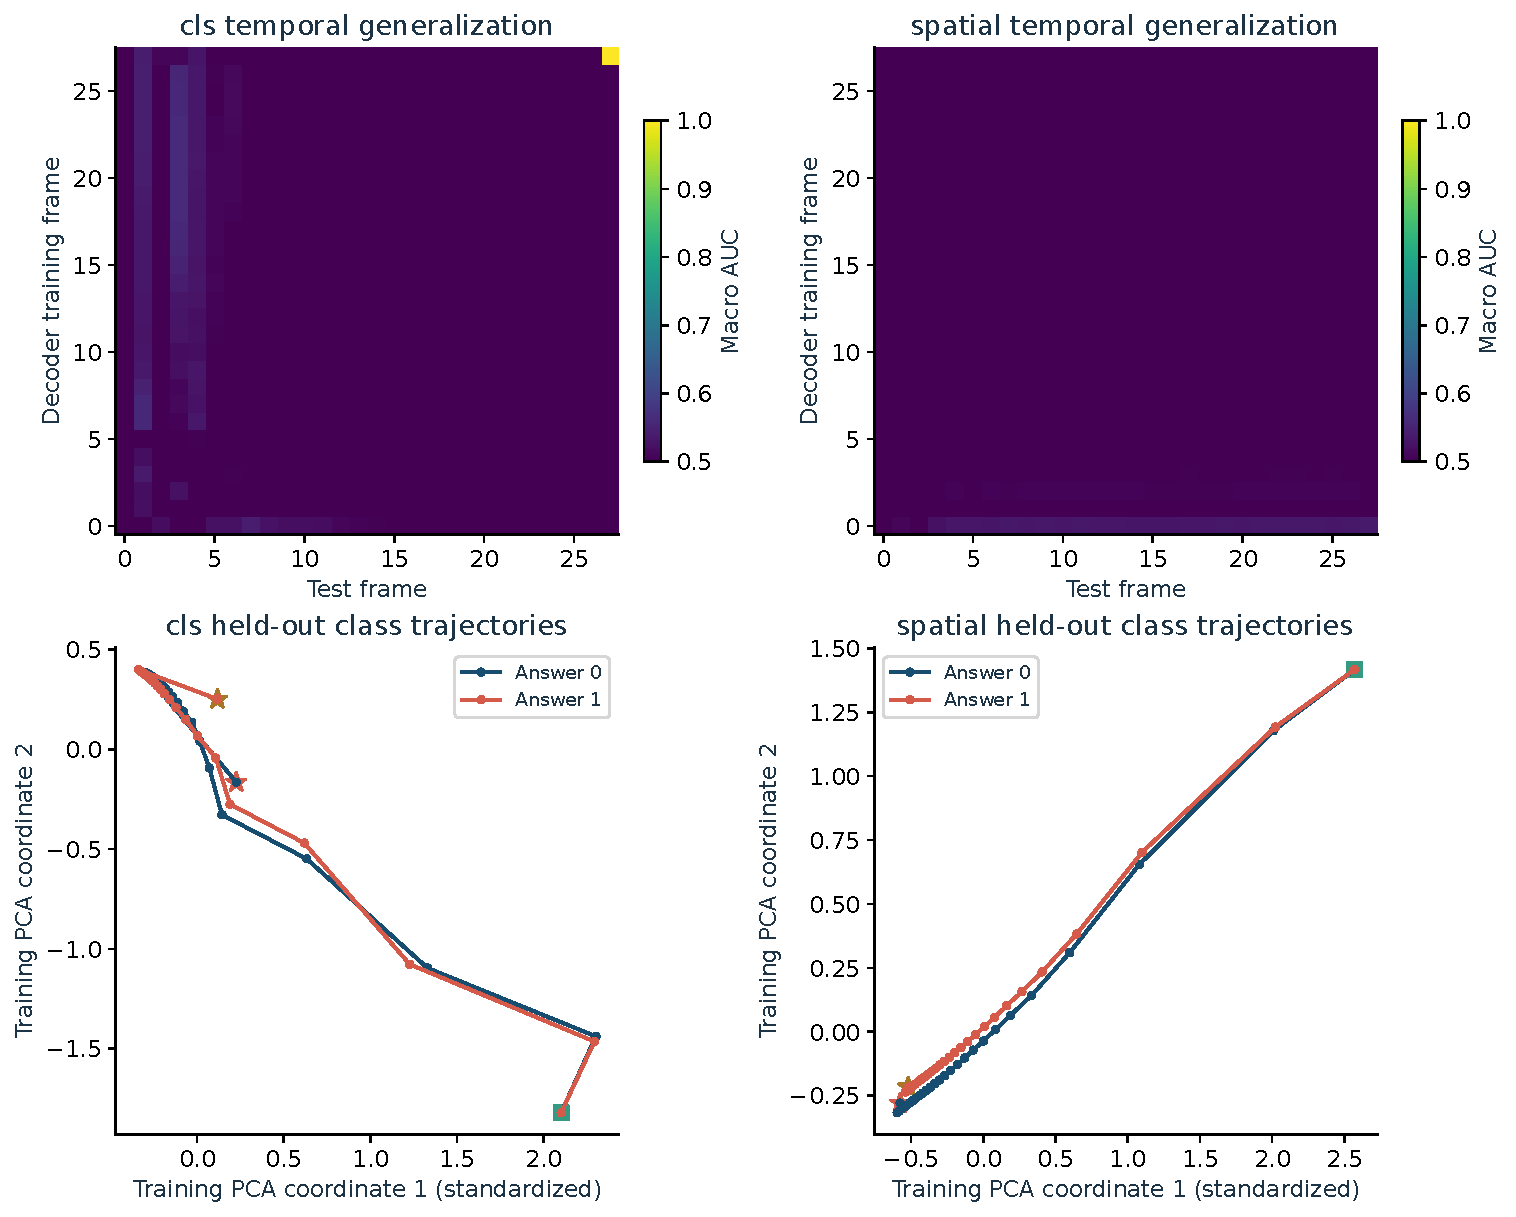
\includegraphics[width=.98\textwidth,height=.65\textheight,keepaspectratio]{../orientation_cued/figures/population.pdf}
\caption{Temporal generalization and held-out population trajectories. Top: decoders fitted separately at each frame and tested across all frames; chance AUC is 0.5. Bottom: class-mean trajectories in a shared training-derived coordinate system, with squares marking starts and stars marking ends. Spatial and CLS populations are analyzed separately.}
\end{figure}
\begin{figure}[htbp]
\centering
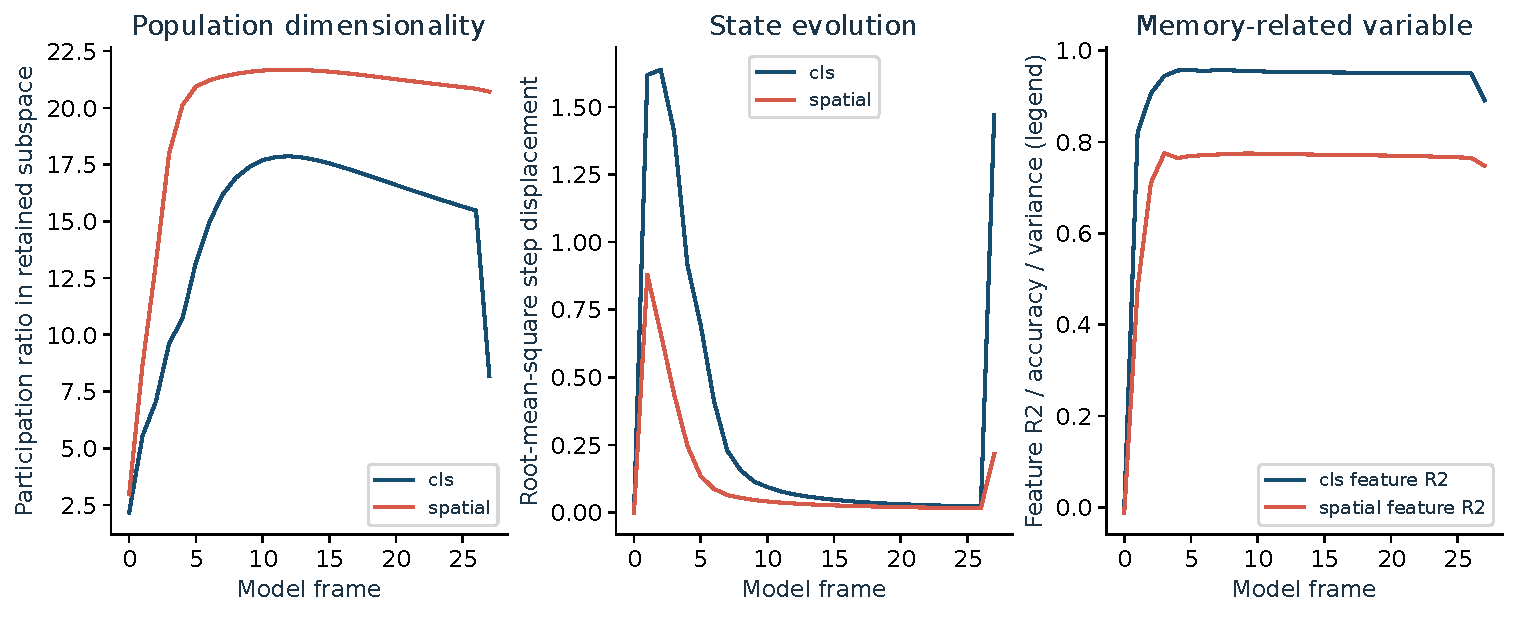
\includegraphics[width=.98\textwidth,height=.65\textheight,keepaspectratio]{../orientation_cued/figures/memory.pdf}
\caption{Population dynamics and mnemonic variables. Left: covariance participation ratio within the retained subspace. Middle: frame-to-frame RMS state displacement. Right: continuous remembered-feature reconstruction when supplied by the task, otherwise location decoding or response-class centroid variance as stated by the legend. Each quantity is tied to the original sequence clock.}
\end{figure}
\subsection{Condition-resolved mechanisms}
The additional panels retain differences between selected stimulus families and timing conditions. Family averages summarize a balanced native factorial; cells remain available individually in the appendix and source data. The decoding comparison uses the same external fitting protocol for every listed condition.

\begin{figure}[htbp]
\centering
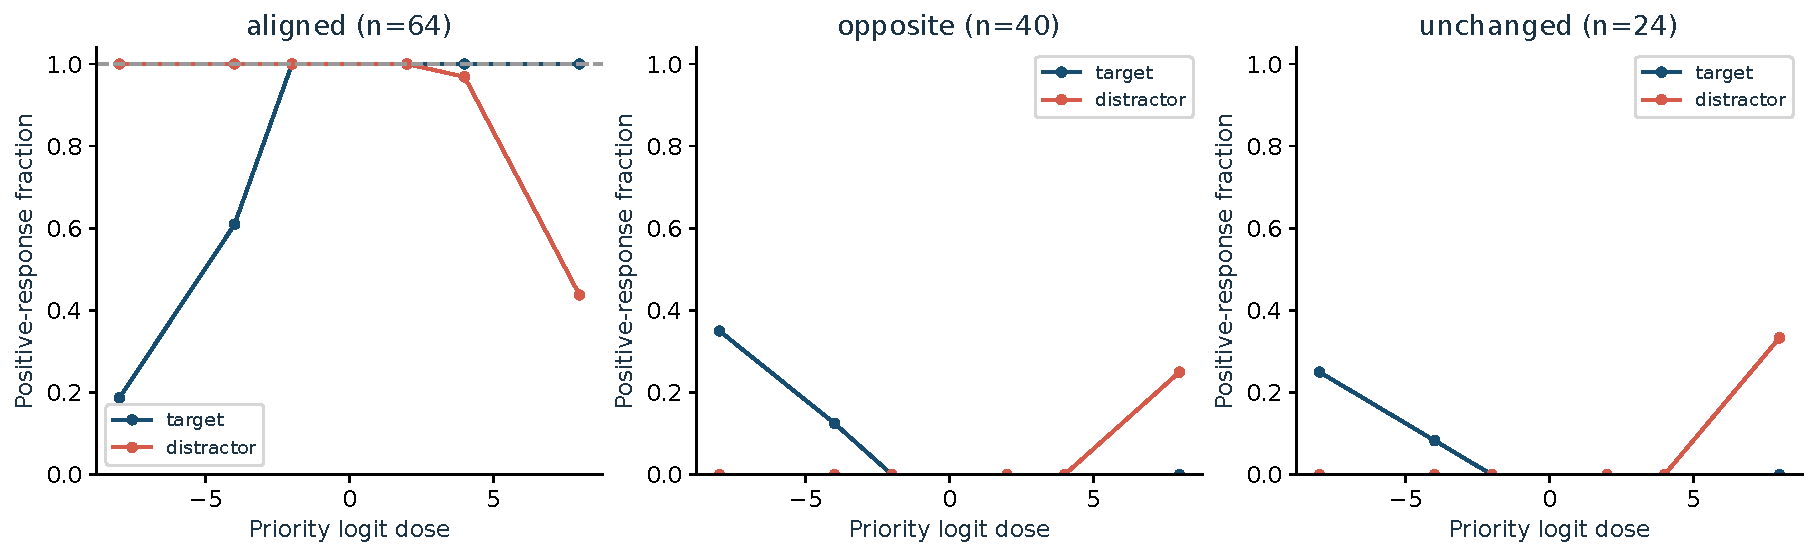
\includegraphics[width=.98\textwidth,height=.65\textheight,keepaspectratio]{../orientation_cued/figures/event_causality.pdf}
\caption{Event-specific causal response functions. Curves show positive reports after evidence-epoch target or alternative-site intervention; the horizontal line is paired sham. Event counts are stated above each panel. A positive report has the task-specific meaning defined in the text.}
\end{figure}
\subsection{Full-state probe control and population selectivity}
\begin{center}\begin{tabular}{lrrr}\toprule Region & Full final AUC & Memory-test AUC & Coordinates\\\midrule
appearance & 0.544 & unavailable & 3200\\
fusion & 0.479 & 0.483 & 6400\\
spatial & 0.617 & 0.434 & 6400\\
cls & 1.000 & 0.418 & 64\\
comparison & 0.487 & 0.499 & 735\\
attention & 0.590 & 0.470 & 100\\
\bottomrule\end{tabular}\end{center}
The full-state control uses the original coordinate width, while the main temporal figures retain at most 32 components. Both evaluations use independent held-out trials. At the final frame, 26 of 64 global-memory units had response-class selectivity at within-population Holm p below 0.05. This is selectivity for the task answer in a recurrent activation coordinate. The complete unit effects and cross-validated centroid-distance trajectories are stored in \texttt{deep\_analysis.json}.

\subsection{Direct verification of attention redistribution}
On 32 exactly replayed trials per selected condition, all six priority arms reproduced their original behavioral probabilities within numerical tolerance. The following figure measures the induced changes in spatial allocation at every frame. This subset supplies a direct map-level manipulation check.
\begin{figure}[htbp]
\centering
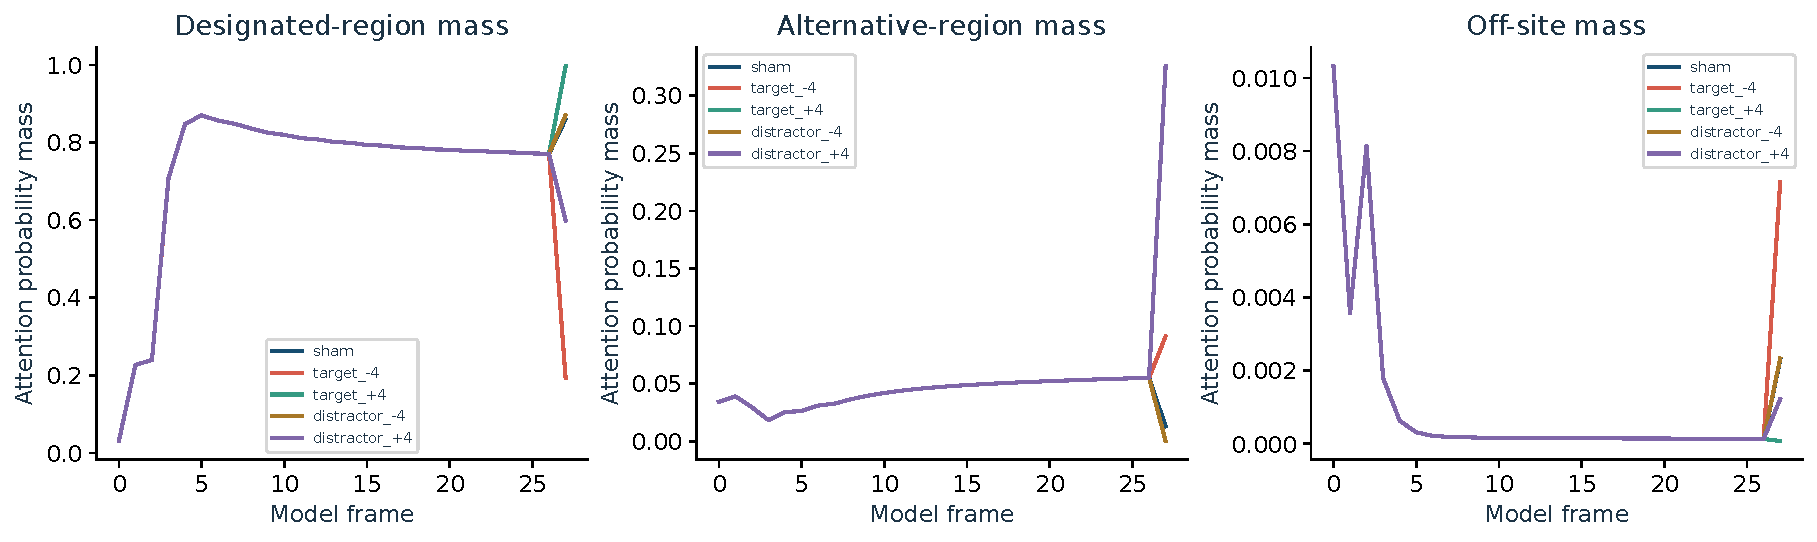
\includegraphics[width=.98\textwidth,height=.65\textheight,keepaspectratio]{../orientation_cued/figures/intervention_maps.pdf}
\caption{Matched map-level verification. Mean designated, alternative and off-site attention mass under sham and four dose-four evidence interventions. These are the first 32 exact movies from the primary intervention experiment, not a new behavioral sample.}
\end{figure}
\subsection{Held-out population response profiles}
The 64 CLS coordinates are ordered by the class with the largest final mean response on fitting trials, with within-class order determined by between-class response variance. The displayed means use independent test trials. Four example coordinates are selected by the largest between-class variance on fitting trials; their held-out trajectories are shown with 1.96 standard-error bands. Activation coordinates use the fitting-set mean and standard deviation across trials and time.

\begin{figure}[htbp]
\centering
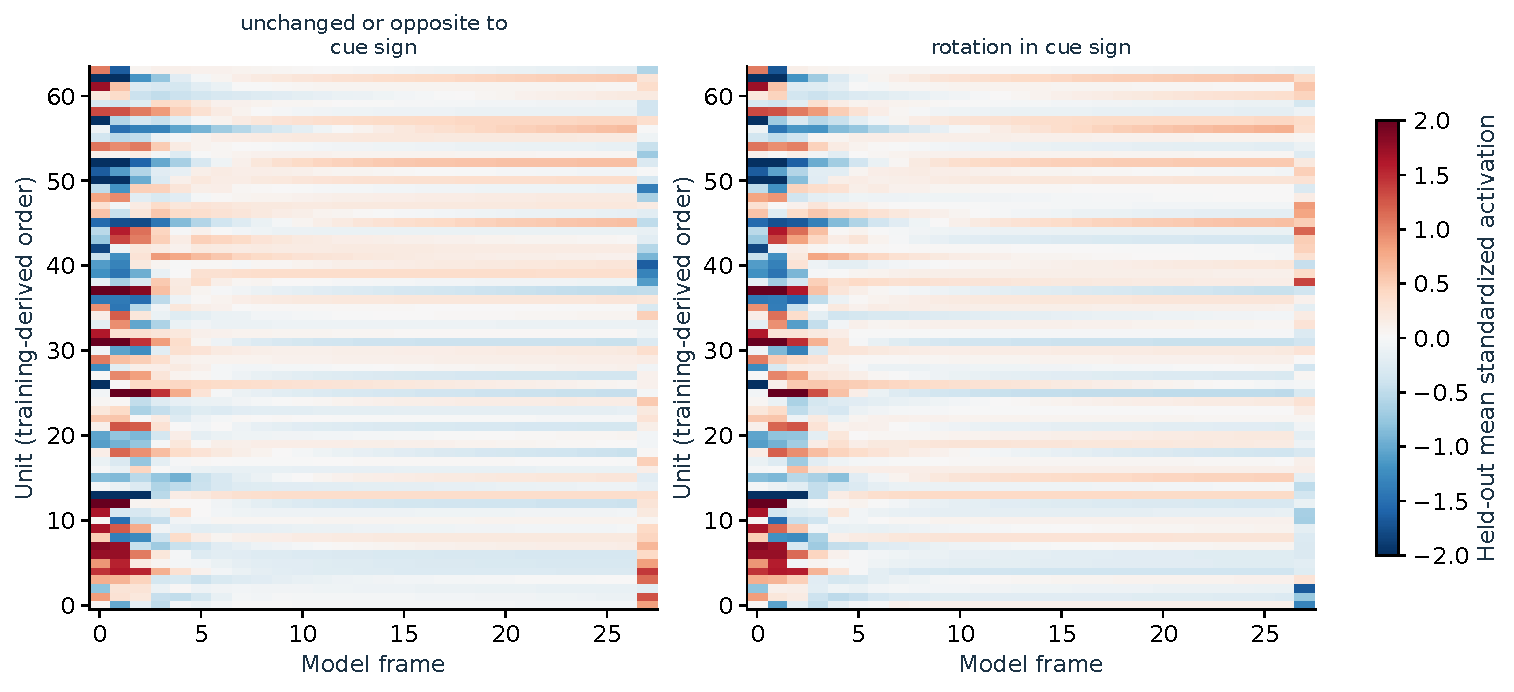
\includegraphics[width=.98\textwidth,height=.65\textheight,keepaspectratio]{../orientation_cued/figures/unit_population.pdf}
\caption{All 64 global-memory coordinates, shown separately for each correct-answer class. Unit ordering and standardization are learned from the fitting population; displayed activity comes from held-out trials. Colors represent activation, not firing rate.}
\end{figure}
\begin{figure}[htbp]
\centering
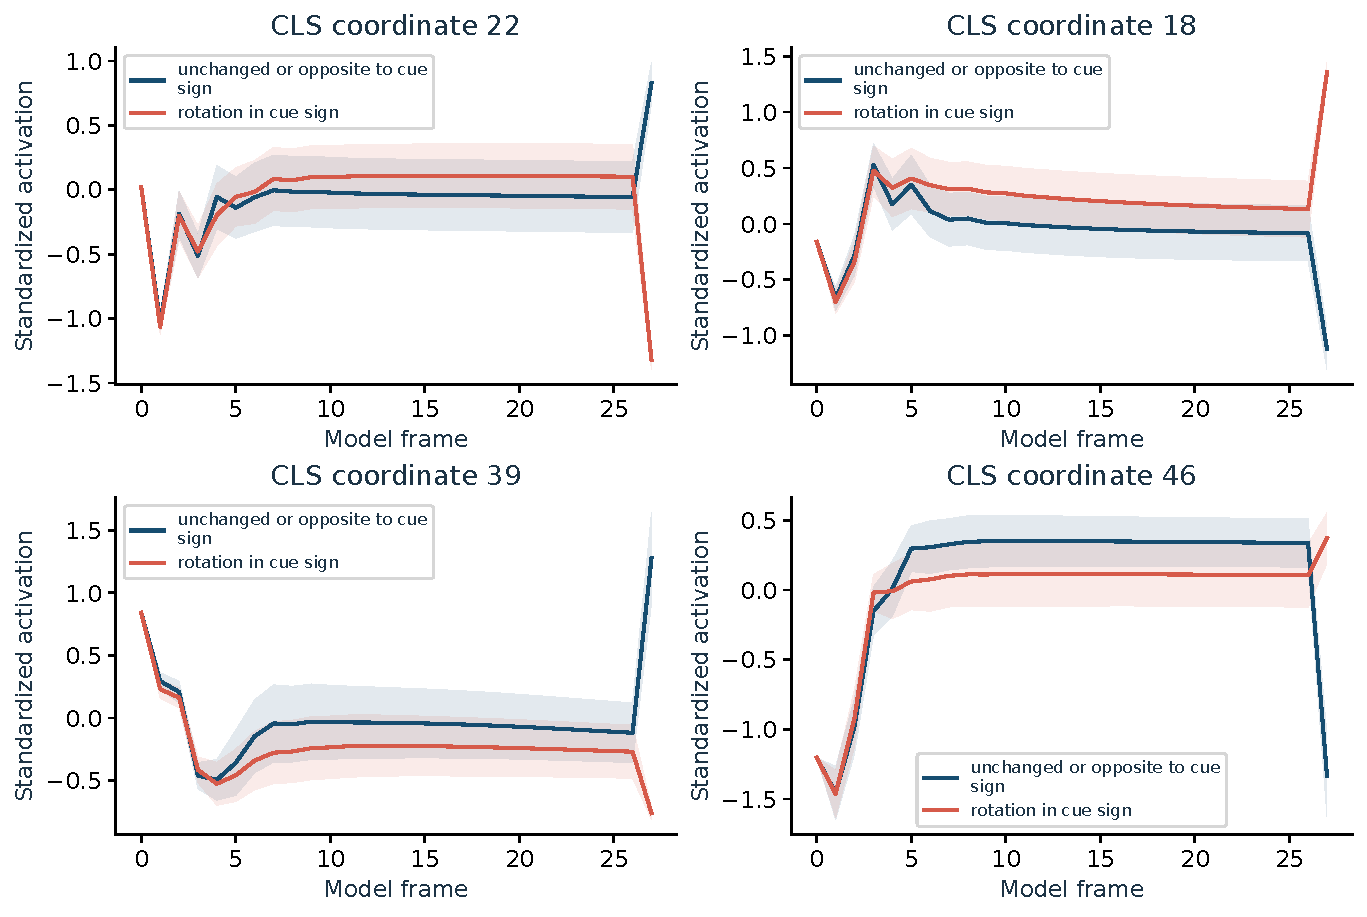
\includegraphics[width=.98\textwidth,height=.65\textheight,keepaspectratio]{../orientation_cued/figures/unit_examples.pdf}
\caption{Four population coordinates selected on fitting trials and evaluated on independent trials. Curves separate response classes; shaded bands describe uncertainty in the mean activation.}
\end{figure}
\subsection{Correct answers, actual choices and spatial instructions}
The correct-answer decoder asks what the stimulus requires; a separate decoder predicts the model's actual terminal choice. They use the same independent fitting/test split and capacity-matched regional features, but distinct target labels. Errors allow these two kinds of information to separate. A location decoder uses the cue index when available, otherwise the instructed or target location. Balanced accuracy averages recall over the labels represented in the held-out population. When every response is correct, answer and choice labels coincide.

\begin{center}\small\begin{tabular}{lrrr}\toprule Region & Correct answer & Actual choice & Cue/target location\\\midrule
appearance & 50.8\% & 50.8\% & 25.8\%\\
fusion & 52.3\% & 52.3\% & 28.1\%\\
spatial & 50.0\% & 50.0\% & 100.0\%\\
cls & 100.0\% & 100.0\% & 66.4\%\\
comparison & 46.1\% & 46.1\% & 53.9\%\\
attention & 57.0\% & 57.0\% & 100.0\%\\
\bottomrule\end{tabular}\normalsize\end{center}
\subsection{Class geometry in the full recurrent states}
For classes $a$ and $b$, let $d^{\rm fit}_j$ and $d^{\rm test}_j$ be their mean-activation differences in coordinate $j$, estimated from independent fitting and test populations and divided by the fitting-set standard deviation at that frame (with a 0.05 floor). The cross-validated distance is $D_{ab}=M^{-1}\sum_{j=1}^{M}d^{\rm fit}_j d^{\rm test}_j$, where $M$ is 64 for global memory and 6,400 for spatial memory. Independent differences remove the positive within-sample noise contribution present when one squared mean difference is used. Negative estimates are retained. Class codes follow the task response labels. This analysis uses every recorded recurrent coordinate and complements the low-dimensional trajectory visualization.

\begin{figure}[htbp]
\centering
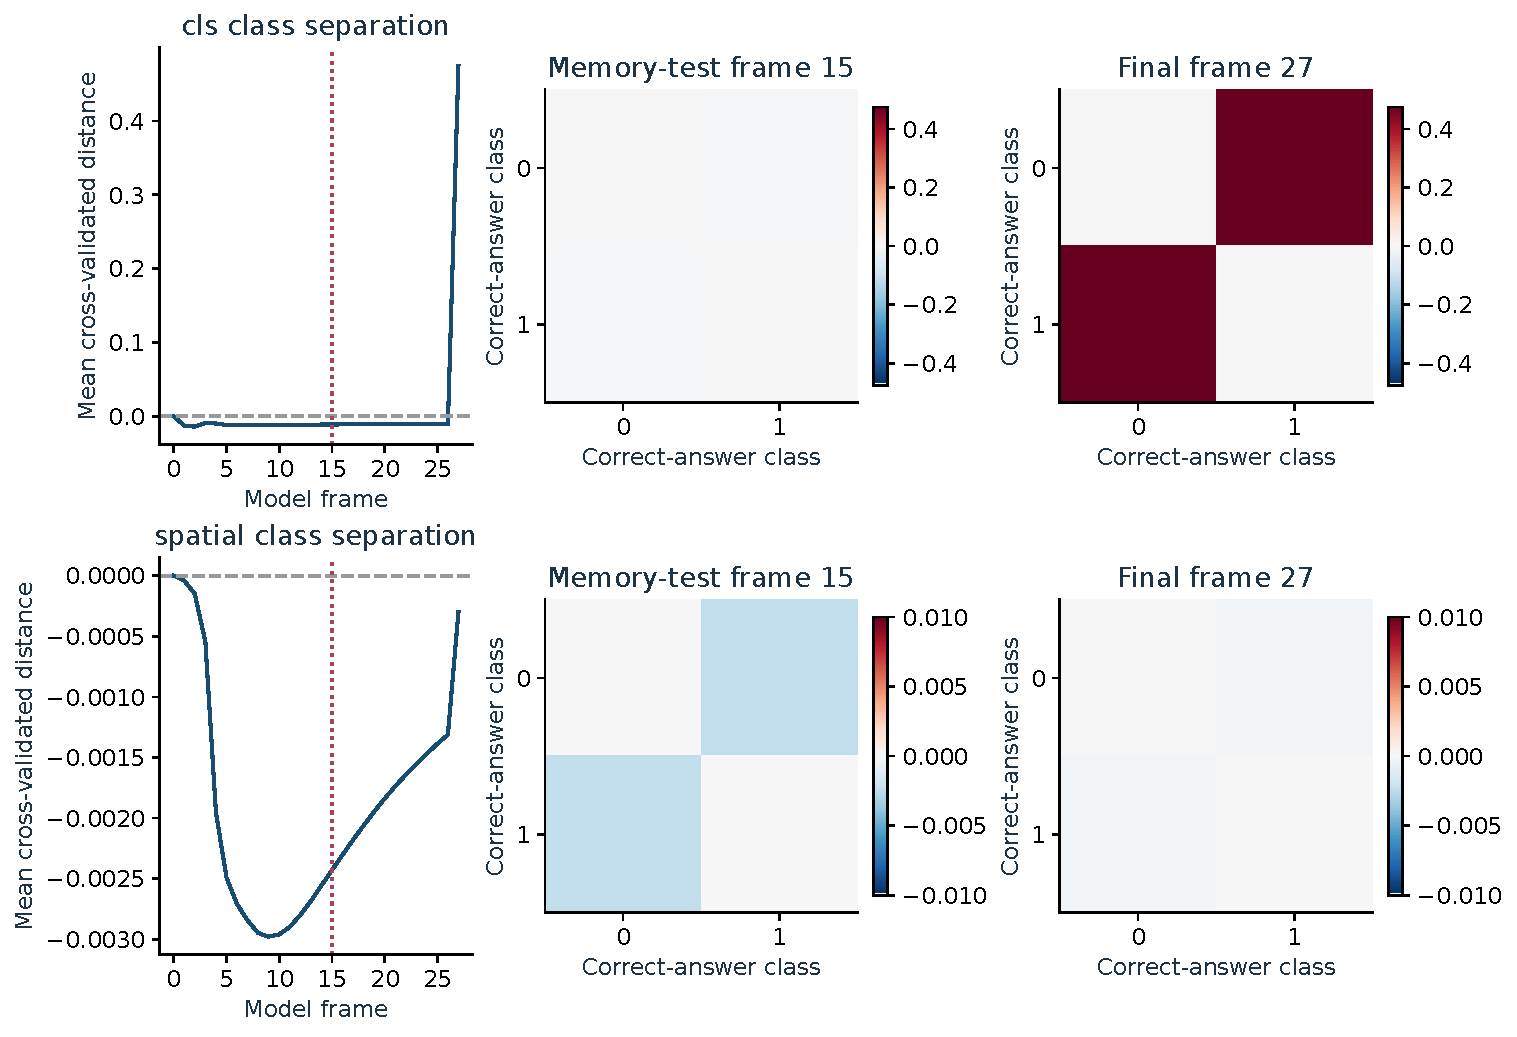
\includegraphics[width=.98\textwidth,height=.65\textheight,keepaspectratio]{../orientation_cued/figures/full_state_geometry.pdf}
\caption{Cross-validated class geometry of the complete recurrent states. Left: mean off-diagonal distance over time, with the memory-test frame marked. Middle and right: class-pair distance matrices at the memory-test and final frames. Color scales are shared between the two matrices within each population. Zero is the null separation baseline; negative estimates remain visible.}
\end{figure}
\subsection{Remembered orientation inventory at all four locations}
A separate content analysis reconstructs all four original sample orientations at every frame. Each orientation angle is encoded as its doubled-angle cosine and sine, respecting the 180-degree periodicity of a grating. The same training-only 32-component representation and ridge penalty used in the main analysis predict the eight continuous target values. Each location has a separate held-out R-squared relative to its fitting-mean predictor. This directly measures location-bound sample content. In the retrospective-cue task, the identity of the eventual target is revealed only after the delay, so all-location reconstruction is the appropriate pre-cue storage measurement.

\begin{figure}[htbp]
\centering
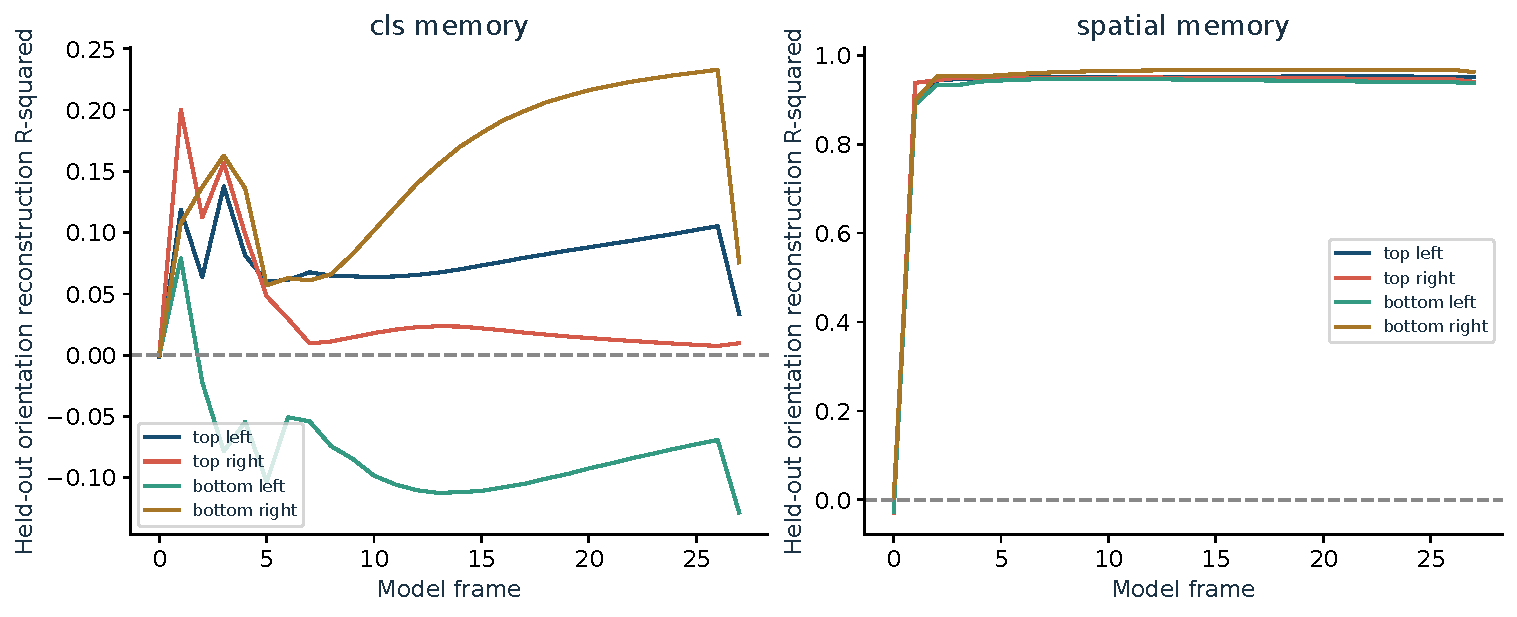
\includegraphics[width=.98\textwidth,height=.65\textheight,keepaspectratio]{../orientation_cued/figures/orientation_inventory.pdf}
\caption{The original orientation at each of the four sample locations decoded from global and spatial memory. Curves track continuous sample content rather than the later correct-answer label. Zero is the fitting-mean baseline.}
\end{figure}
\clearpage\section{Discussion}
The continuous-feature analysis and the response-label analysis describe different stages of the task. Sample orientation remains readable during the delay, whereas the final answer depends on the later rotation and cue rule. A mid-delay spatial reset causes a large subsequent accuracy loss, while the same-time global reset produces no observed loss in this sample. The latter state can be reconstructed during the remaining frames from information still available elsewhere. Target inhibition at the probe separately demonstrates a causal selection requirement. The combined result supports a sequence of retained spatial content, later selection, and rule-dependent response construction.

The behavioral result establishes 99.8\% native accuracy for this trained subject across the tested condition distribution. The information result identifies cls as the strongest final regional readout in the representative condition under the fixed probe procedure. The causal result identifies target\_\allowbreak{}-8\_\allowbreak{}evidence as the largest observed impairment in that condition. These three findings concern distinct levels of explanation: successful behavior, recoverable information and dependence on a manipulated component. Their conjunction is more informative than any one alone.

The most useful interpretation of a null manipulation is determined by its interval and by whether it altered an active component at a relevant time. Zero-active-frame interventions are identified in the data, and comparison memory can be exactly zero in short sequences. The shared softmax also makes priority changes competitive: increasing one region necessarily changes the relative mass elsewhere. Thus the causal object is the complete redistribution induced by the specified intervention.

A full factorial of cue sign, target rotation and foil congruence would distinguish mnemonic degradation from rule confusion. Applying a late countercue would test how rapidly the stored representation can be read under a different instruction.

% BEGIN BIOLOGICAL DISCUSSION
\subsection{Interpreting these results alongside biological experiments}
\subsubsection{Harrison and Tong (2009)}
Sample orientation is readable during the model’s delay, matching the key computational observation that absent visual content can remain available in a population pattern. The model adds a causal intervention: resetting spatial memory during retention causes a large later cost. This links information availability to behavior more directly than a decoder alone. \cite{bio_harrison}

\subsubsection{Griffin and Nobre (2003)}
The cue determines which retained content or location matters for a subsequent comparison. The human cue experiments motivate separating a benefit at encoding from selection within memory. In this model, probe-period target inhibition provides a later selection test, while the delay reset tests retention. Their separate effects support distinct stages of the computation. \cite{bio_griffin}

\subsubsection{Stokes and colleagues (2013)}
The model’s answer becomes meaningful only after the probe and rule define it. A population can therefore transform from an orientation code into a decision code. Cross-temporal decoding tests whether one linear readout remains useful across those phases. A changing geometry can support stable task performance when the downstream computation reads the appropriate phase-dependent state. \cite{bio_stokes}

\subsection{A computational account of the observed behavior}
The crucial theoretical distinction is between storing a stimulus and storing a response. Before the probe, the network can retain sample orientation and spatial context; after the probe it can compute a signed rotation and apply the required rule. The large spatial reset cost localizes a necessary retained contribution. The absence of a measured cost from a global reset at the same instant has a narrower interpretation: global state can be restored or bypassed using other remaining state during the subsequent frames. It does not imply that global memory never participates. The time-resolved maps and decoder matrices make these stages visible: encoding, retention, renewed sensory selection and final response construction.

\subsection{Where this task agrees with the biological evidence}
The model agrees with retained sensory content and subsequent attentional selection. Its division of labor favors spatial memory at the tested delay time. The biological theory of dynamic coding becomes a testable account when content decoders transfer differently across phases while the causal dependence on the stored information remains.

\subsection{A follow-up experiment motivated by these results}
Apply brief resets at multiple delay times and immediately before the probe. Decode the sample angle after each reset, then measure whether behavior recovers. Separate rapid reconstruction from true tolerance to loss of the represented orientation.
% END BIOLOGICAL DISCUSSION
\subsection{Scope of inference}
This series studies one trained parameter realization. Its uncertainty intervals describe stimulus sampling for that realization. Threshold-defined latencies are in model frames and reflect the existing classifier applied to prefix states. Spatial doses are changes to computational priority logits, and memory perturbations act on recurrent tensors. Independent training seeds, calibrated behavioral clocks and biological intervention models are the next levels of replication. The empirical results, code and task definitions are sufficient to reproduce the computational experiments reported here.

\begin{thebibliography}{99}
\bibitem{spatial} Funahashi S, Bruce CJ, Goldman-Rakic PS (1989). Mnemonic coding of visual space in the monkey dorsolateral prefrontal cortex. Journal of Neurophysiology 61:331-349. \url{https://pubmed.ncbi.nlm.nih.gov/2918358/}.
\bibitem{stokes} Stokes MG et al. (2013). Dynamic coding for cognitive control in prefrontal cortex. Neuron 78:364-375. \url{https://pubmed.ncbi.nlm.nih.gov/23562541/}.
\bibitem{king} King JR, Dehaene S (2014). Characterizing the dynamics of mental representations: the temporal generalization method. Trends in Cognitive Sciences 18:203-210. \url{https://pmc.ncbi.nlm.nih.gov/articles/PMC5635958/}.
% BEGIN BIOLOGICAL REFERENCES
\bibitem{bio_harrison} Harrison and Tong (2009). Decoding reveals the contents of visual working memory in early visual areas. \href{https://pubmed.ncbi.nlm.nih.gov/19225460/}{Primary source}.
\bibitem{bio_griffin} Griffin and Nobre (2003). Orienting attention to locations in internal representations. \href{https://pubmed.ncbi.nlm.nih.gov/14709235/}{Primary source}.
\bibitem{bio_stokes} Stokes and colleagues (2013). Dynamic coding for cognitive control in prefrontal cortex. \href{https://pmc.ncbi.nlm.nih.gov/articles/PMC3898895/}{Primary source}.
% END BIOLOGICAL REFERENCES
\end{thebibliography}\clearpage\appendix\section{Complete native condition results}
\small\begin{longtable}{p{.44\textwidth}rrrr}\toprule Condition & n & Accuracy & AUC & Brier\\\midrule\endhead
D0 & 128 & 100.0\% & 1.000 & 0.001\\
D4 & 128 & 100.0\% & 1.000 & 0.000\\
D12 & 128 & 100.0\% & 1.000 & 0.000\\
D24 & 128 & 99.2\% & 1.000 & 0.009\\
\bottomrule\end{longtable}\normalsize\section{Every-frame attention atlas}
Condition D24. The first two rows show one exact native trial and its own attention overlay. The third row averages attention over 16 trials sharing the selected location/cue and response label. Every model frame is included. Averaging unrelated object identities is restricted to the attention map; the displayed RGB movie remains one real trial.
\begin{figure}[htbp]
\centering
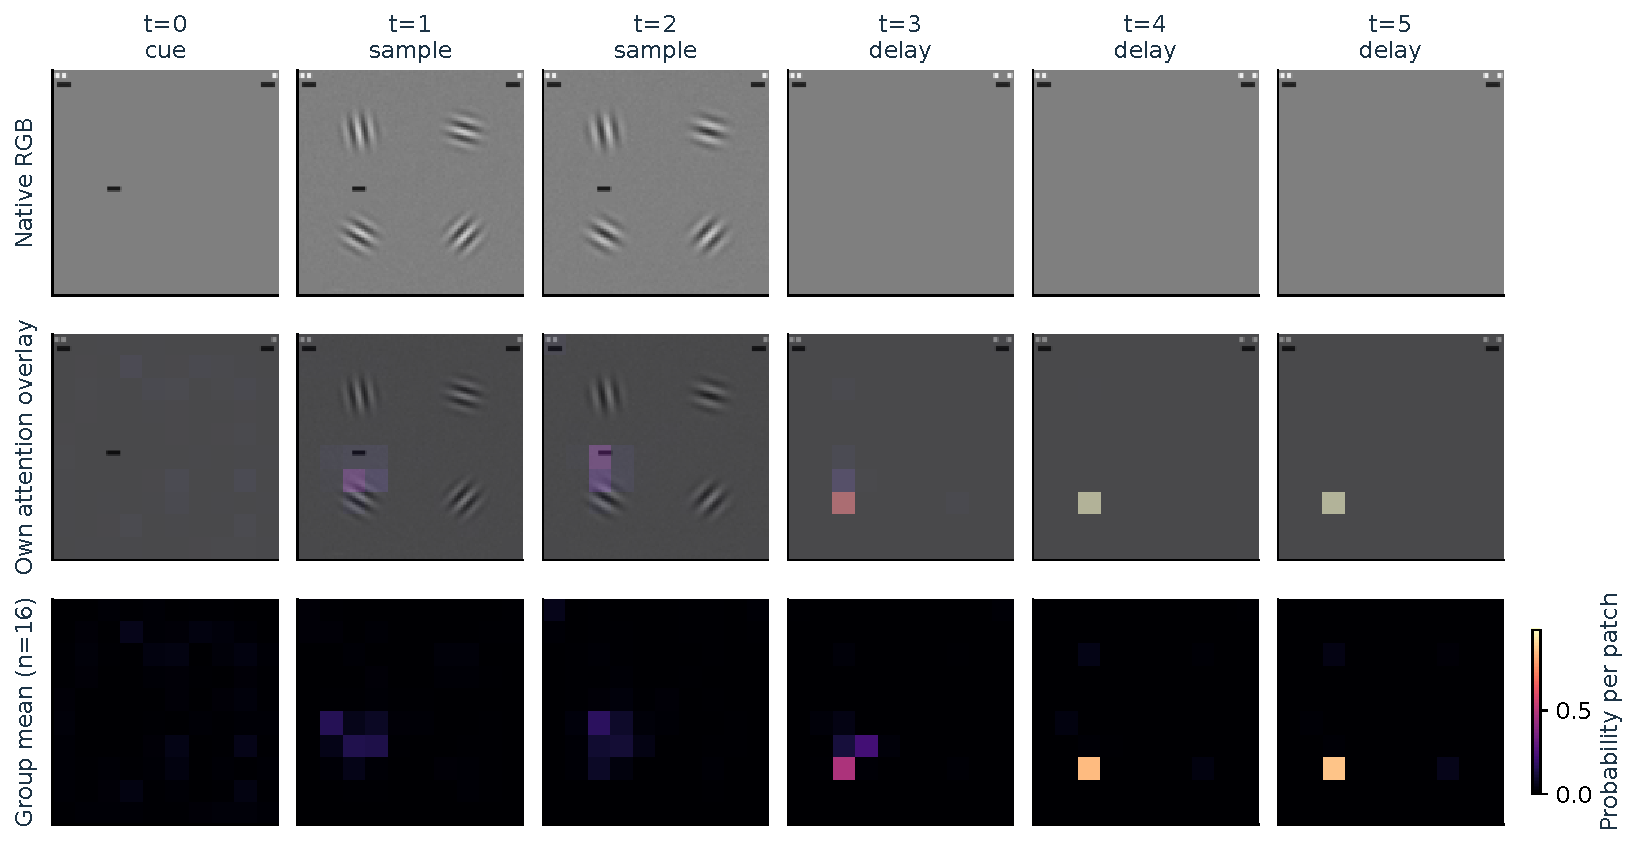
\includegraphics[width=.98\textwidth,height=.65\textheight,keepaspectratio]{../orientation_cued/figures/atlas_000.pdf}
\caption{Native frames, own attention overlay and condition-group spatial projection. Shared color scaling within each panel represents attention probability per patch.}
\end{figure}
\begin{figure}[htbp]
\centering
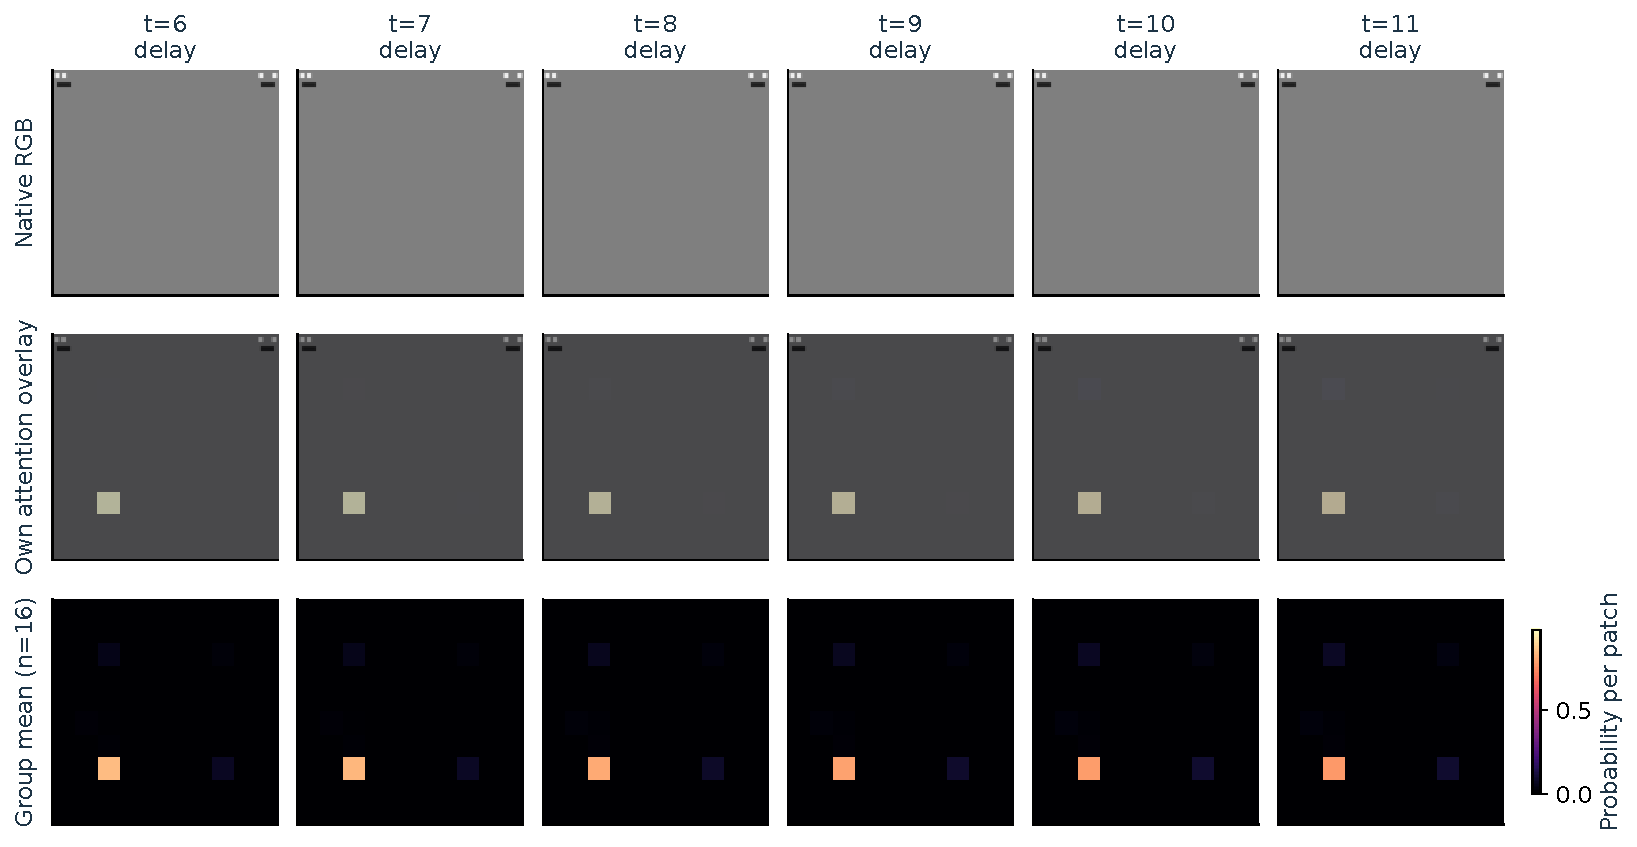
\includegraphics[width=.98\textwidth,height=.65\textheight,keepaspectratio]{../orientation_cued/figures/atlas_006.pdf}
\caption{Native frames, own attention overlay and condition-group spatial projection. Shared color scaling within each panel represents attention probability per patch.}
\end{figure}
\begin{figure}[htbp]
\centering
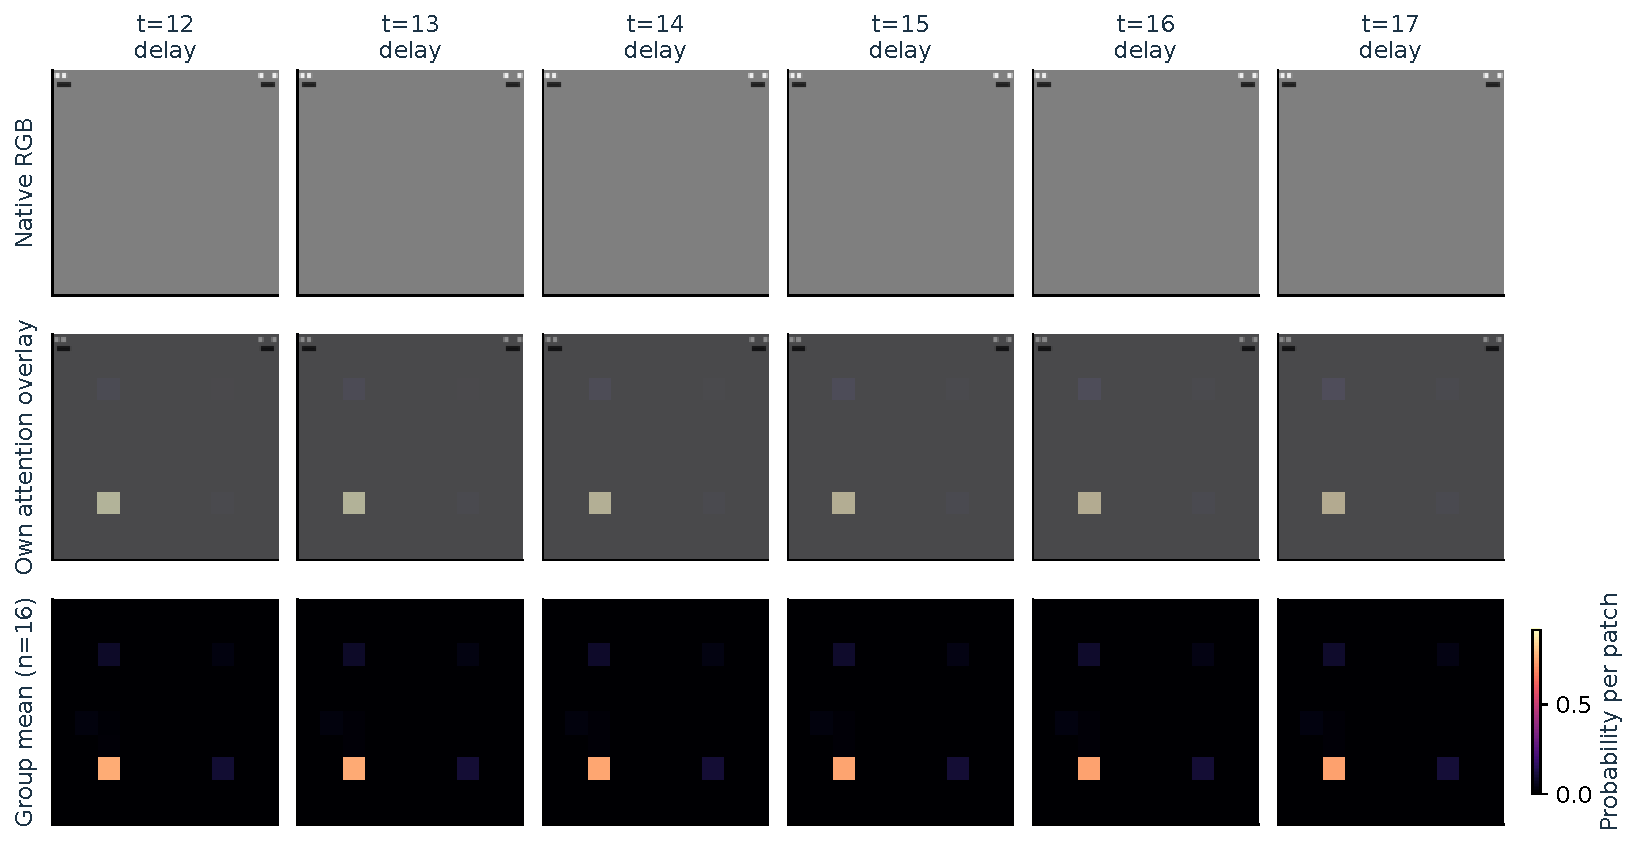
\includegraphics[width=.98\textwidth,height=.65\textheight,keepaspectratio]{../orientation_cued/figures/atlas_012.pdf}
\caption{Native frames, own attention overlay and condition-group spatial projection. Shared color scaling within each panel represents attention probability per patch.}
\end{figure}
\begin{figure}[htbp]
\centering
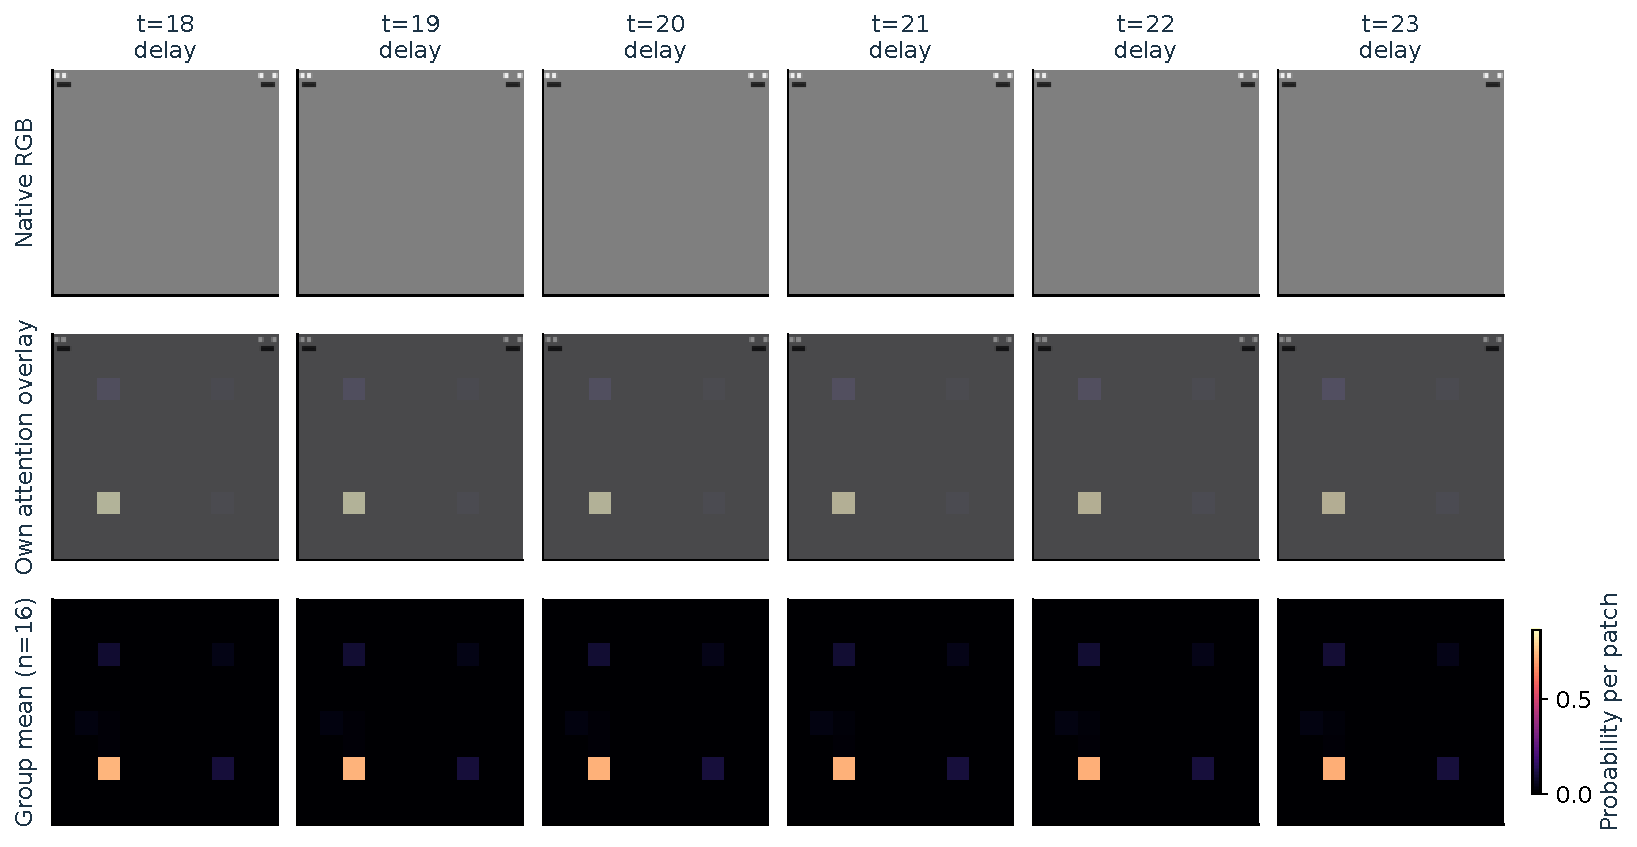
\includegraphics[width=.98\textwidth,height=.65\textheight,keepaspectratio]{../orientation_cued/figures/atlas_018.pdf}
\caption{Native frames, own attention overlay and condition-group spatial projection. Shared color scaling within each panel represents attention probability per patch.}
\end{figure}
\begin{figure}[htbp]
\centering
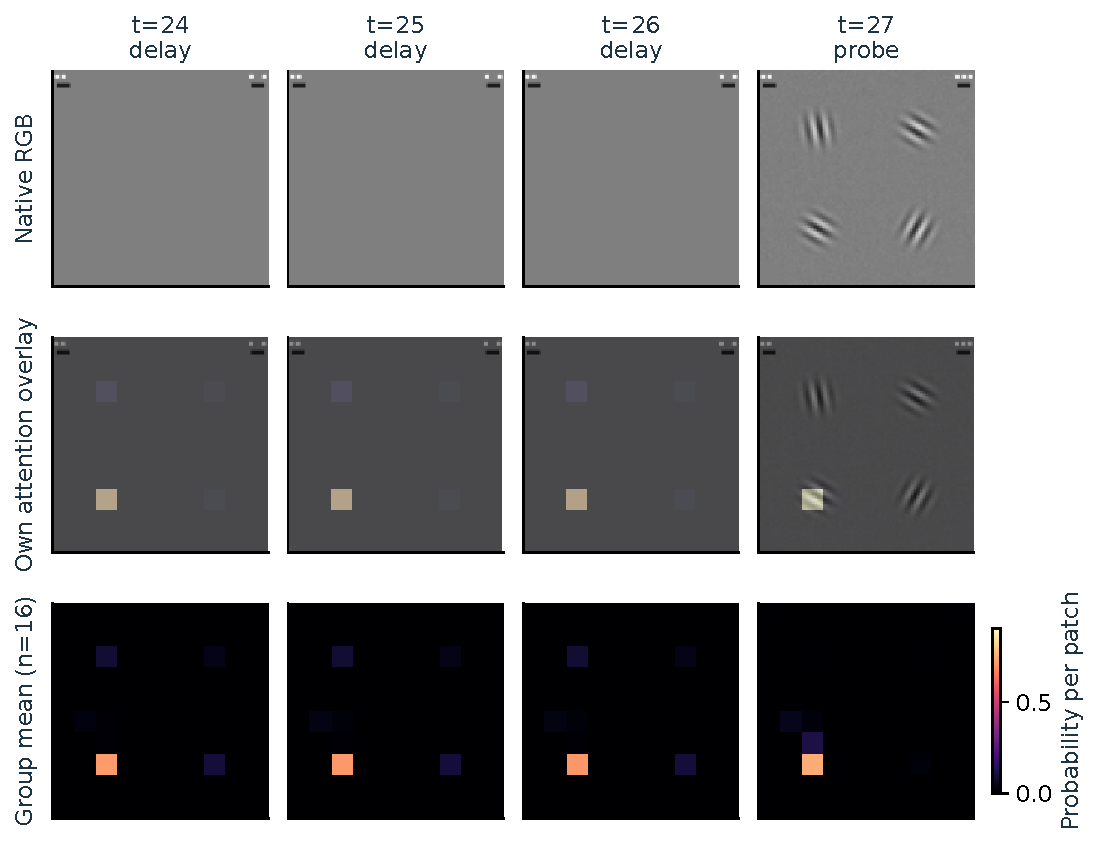
\includegraphics[width=.98\textwidth,height=.65\textheight,keepaspectratio]{../orientation_cued/figures/atlas_024.pdf}
\caption{Native frames, own attention overlay and condition-group spatial projection. Shared color scaling within each panel represents attention probability per patch.}
\end{figure}
% BEGIN FULL CONDITION ATTENTION
\clearpage\section{Condition-by-time attention: all frames}
Each panel retains the same condition definitions and color scale as the main attention section. Frames are aligned to the task-specific evidence onset. Gray cells mark times outside a particular trial, rather than missing observations. All observed frames are displayed.
\clearpage
\begin{figure}[htbp]
\centering
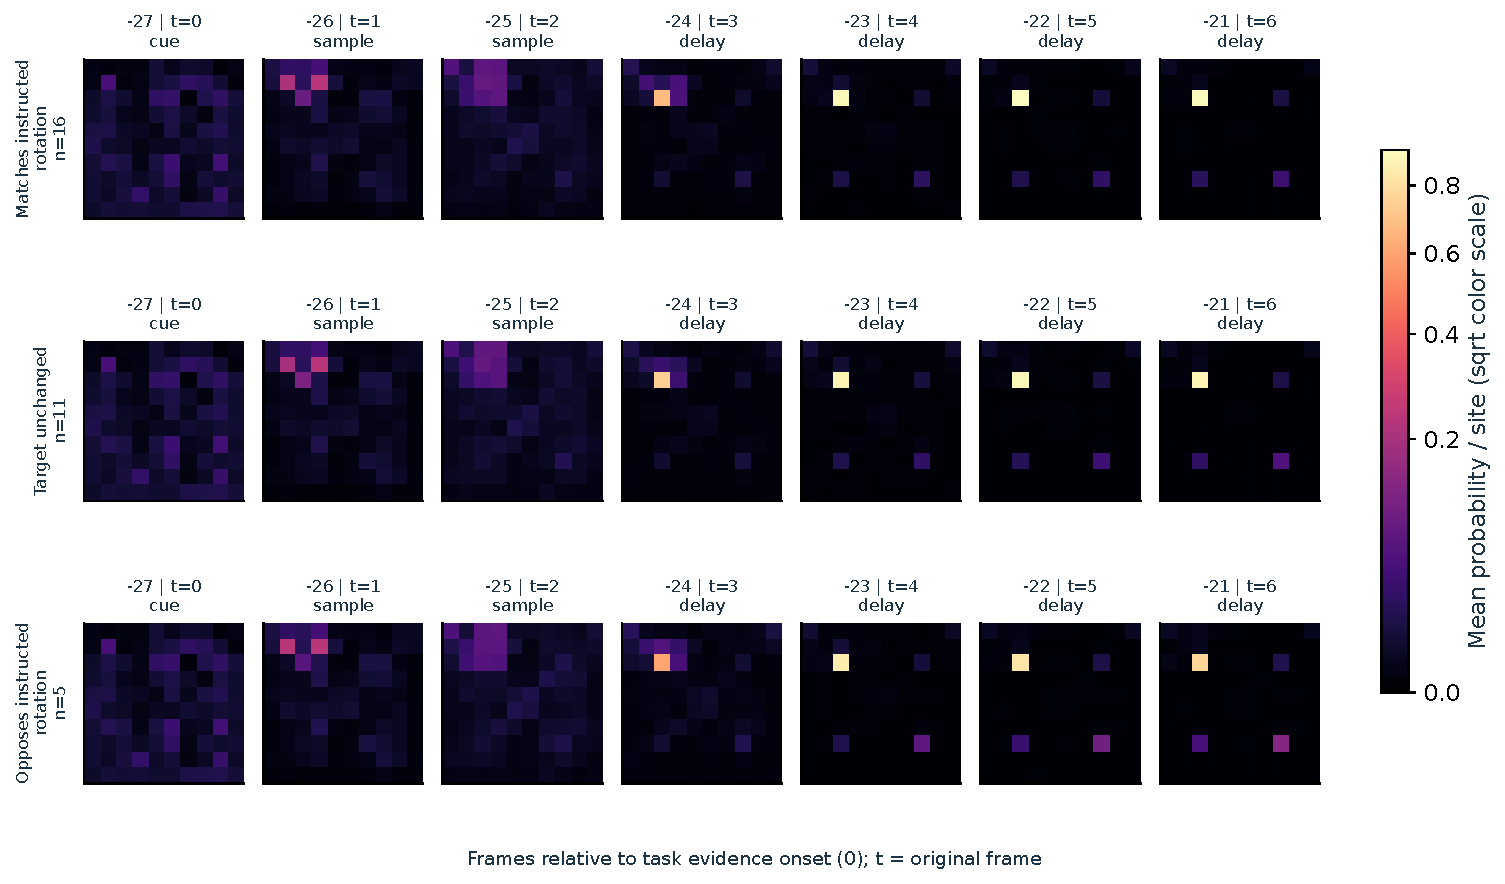
\includegraphics[width=.98\textwidth,height=.65\textheight,keepaspectratio]{../orientation_cued/figures/attention_conditions_maps_00_000.pdf}
\caption{Complete condition-average spatial trajectory. Rows are conditions, columns are aligned frames, and each title also records the original frame and task phase. Sample counts and a shared probability scale accompany every panel.}
\end{figure}
\clearpage
\begin{figure}[htbp]
\centering
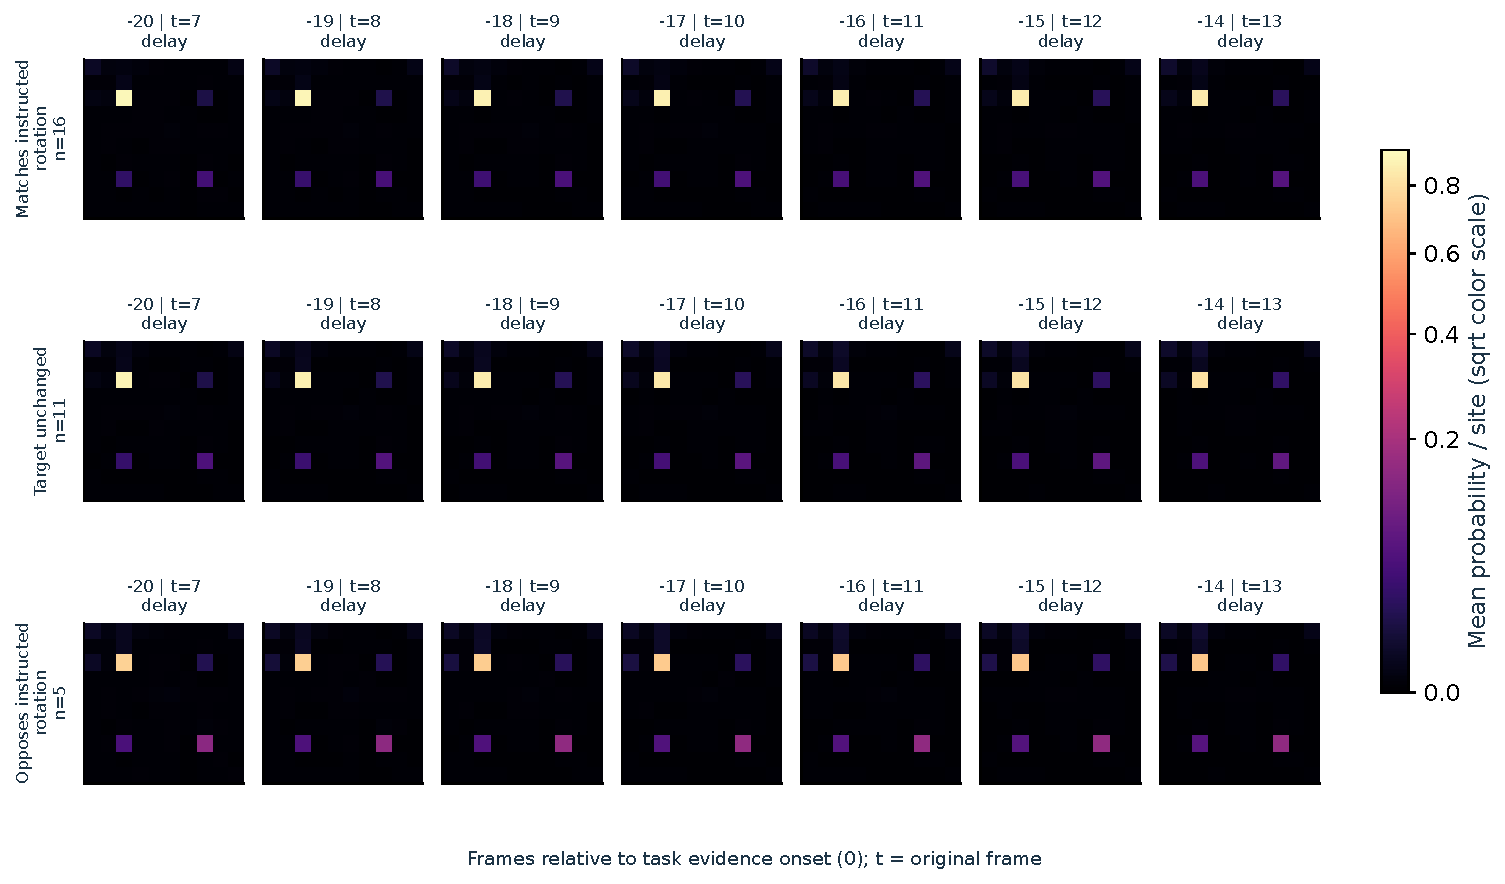
\includegraphics[width=.98\textwidth,height=.65\textheight,keepaspectratio]{../orientation_cued/figures/attention_conditions_maps_00_007.pdf}
\caption{Complete condition-average spatial trajectory. Rows are conditions, columns are aligned frames, and each title also records the original frame and task phase. Sample counts and a shared probability scale accompany every panel.}
\end{figure}
\clearpage
\begin{figure}[htbp]
\centering
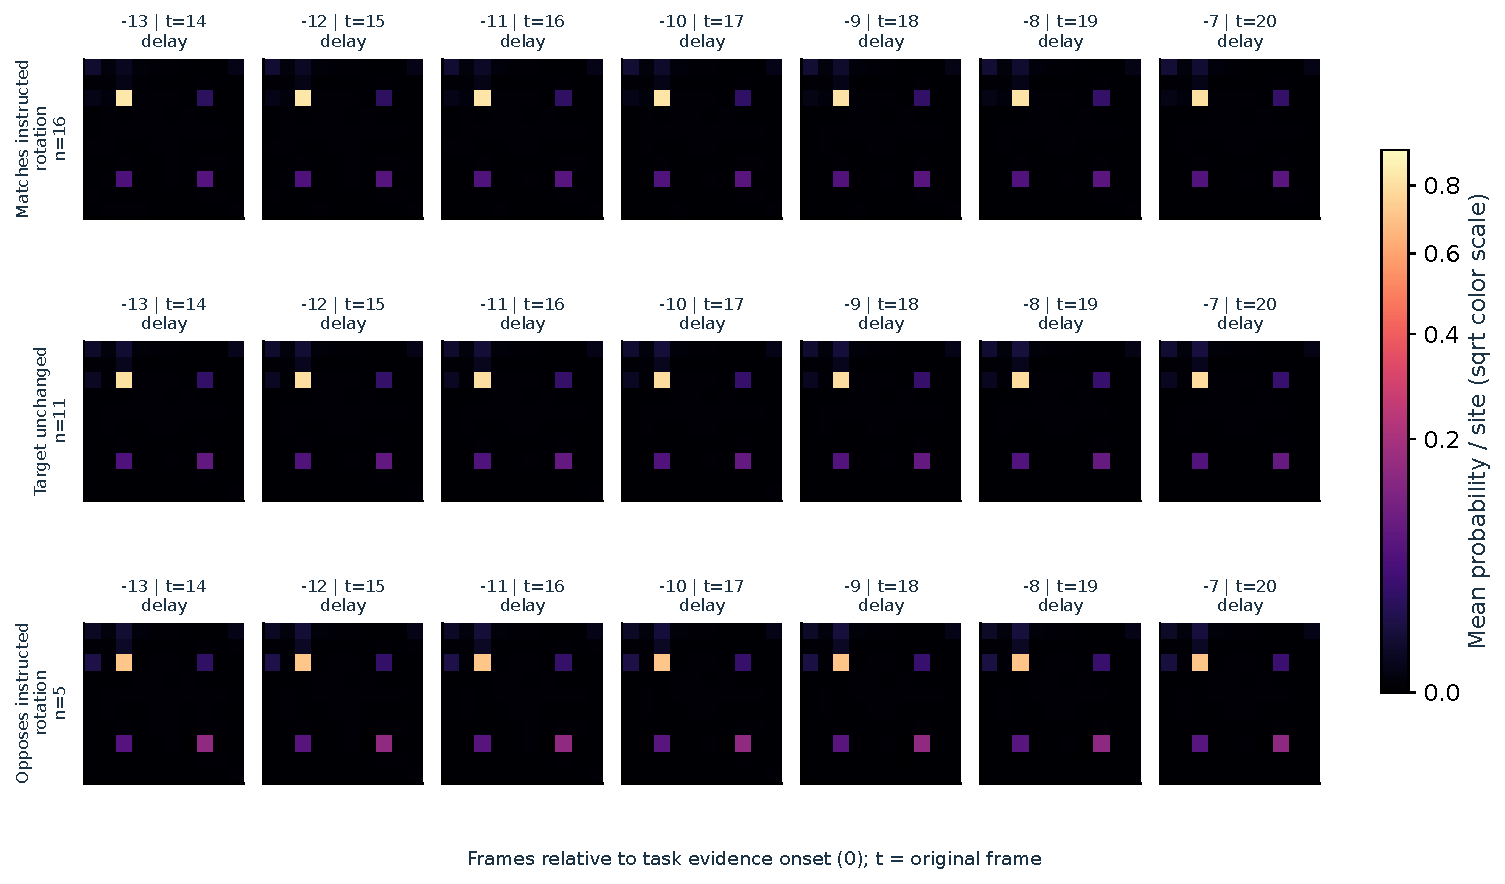
\includegraphics[width=.98\textwidth,height=.65\textheight,keepaspectratio]{../orientation_cued/figures/attention_conditions_maps_00_014.pdf}
\caption{Complete condition-average spatial trajectory. Rows are conditions, columns are aligned frames, and each title also records the original frame and task phase. Sample counts and a shared probability scale accompany every panel.}
\end{figure}
\clearpage
\begin{figure}[htbp]
\centering
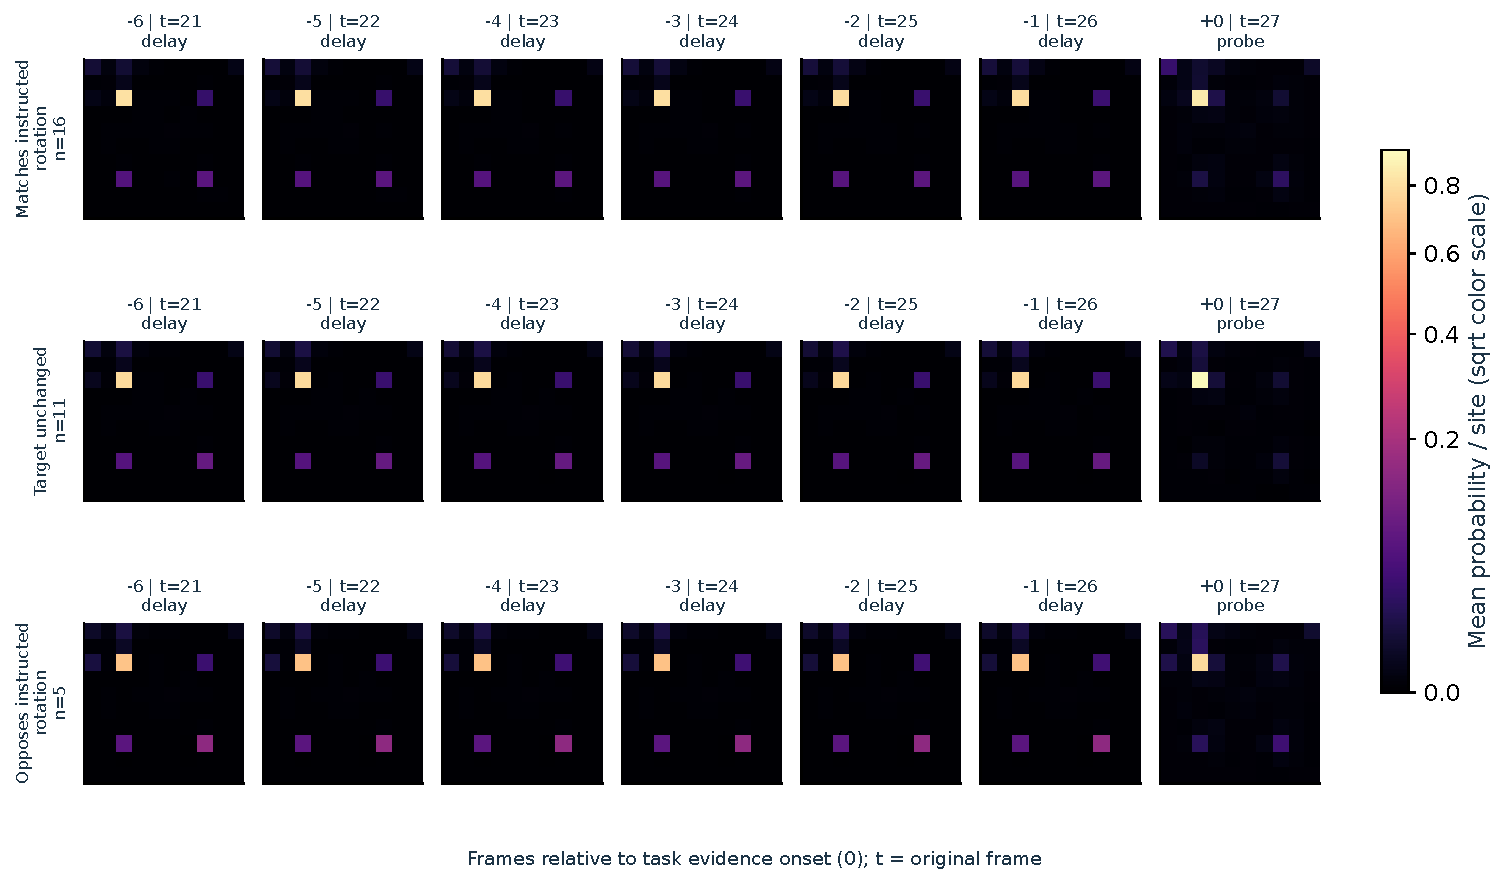
\includegraphics[width=.98\textwidth,height=.65\textheight,keepaspectratio]{../orientation_cued/figures/attention_conditions_maps_00_021.pdf}
\caption{Complete condition-average spatial trajectory. Rows are conditions, columns are aligned frames, and each title also records the original frame and task phase. Sample counts and a shared probability scale accompany every panel.}
\end{figure}
% END FULL CONDITION ATTENTION
\clearpage\section{Reproducibility record}
Main checkpoint: update 204,289. Final robustness checkpoint: update 220,637.

best: \texttt{596bc351783b3ddbfa8d37a9cf8d6514}\par\texttt{6d1333dcc0097d40f0f75665b6451bcf}

latest: \texttt{c13338ff6958c5dbb617914da538bca1}\par\texttt{39944b89122b848b72885ed3241995d4}

Data namespace 205903; probe fitting 205904; probe testing 205905; interventions 205906; difficulty challenges 205907; VDA counterfactuals 205908. The analysis package is \texttt{SecondPass/TaskNeuroscience}. The protocol, source hashes, parity checks, per-trial NPZ files, metadata, statistical JSON files and editable LaTeX sources are retained beside this paper. Figures and text are generated directly from completed analysis results.
\end{document}